\setcounter{secnumdepth}{4}
\lstdefinestyle{csharp}{
    language=C#,
    basicstyle=\ttfamily\small,
    commentstyle=\color{green!40!black},
    keywordstyle=\color{blue},
    numberstyle=\tiny\color{gray},
    numbers=left,
    stepnumber=1,
    numbersep=5pt,
    backgroundcolor=\color{white},
    showspaces=false,
    showstringspaces=false,
    showtabs=false,
    tabsize=2,
    frame=single,
    rulecolor=\color{black},
    captionpos=b,
    breaklines=true,
    breakatwhitespace=false,
    title=\lstname,
    escapeinside={\%*}{*)},
    morekeywords={var},
}

\chapter{Feinkonzept und Realisierung}

\section{Entwicklungsumgebungen}
\subsection{Visual Studio 2022}
Visual Studio 2022 ist eine integrierte Entwicklungsumgebung (IDE) von Microsoft, die speziell für die Entwicklung von
Softwareanwendungen, Webanwendungen und Desktop-Anwendungen konzipiert ist. Es handelt sich um eine umfangreiche
Entwicklungsumgebung, die von Entwicklern weltweit für eine breite Palette von Anwendungsfällen eingesetzt wird.

\subsection{Unity}
Der Unity-Editor, entwickelt von Unity Technologies, fungiert als umfassende integrierte Entwicklungsumgebung (IDE)
und zentrale Arbeitsumgebung für die Konzeption und Umsetzung von 2D-, 3D-, Augmented Reality (AR) und Virtual Reality
(VR) Anwendungen und Spielen. Als Kernelement der Unity-Plattform spielt der Editor eine entscheidende Rolle in der
Entwicklung von Projekten, die auf Unity-Technologien basieren.

Die Funktionalität des Unity-Editors erstreckt sich über verschiedene Aspekte der Softwareentwicklung, angefangen bei
der visuellen Gestaltung von Szenen und Spielwelten bis hin zur Implementierung komplexer Logik und Interaktionen. Die
folgenden Abschnitte vertiefen die Schlüsselmerkmale und Funktionen des Unity-Editors, die ihn zu einem essenziellen
Werkzeug für Entwickler machen.

\subsubsection{Multidisziplinäre Unterstützung und Integration}
Der Unity-Editor zeichnet sich durch seine multidisziplinäre Unterstützung aus, die Entwicklern ermöglicht, kollaborativ
an Projekten zu arbeiten. Künstler, Entwickler und Designer können innerhalb derselben Umgebung zusammenarbeiten,
wodurch ein nahtloser Austausch von Assets, Szenen und Ressourcen ermöglicht wird. Die Integration von Grafik-,
Physik- und Audio-Engines erleichtert die Schaffung immersiver und ansprechender digitaler Umgebungen.

\subsubsection{Szenengestaltung und Asset-Management}
Ein zentrales Merkmal des Unity-Editors ist die intuitive Szenengestaltung, die es Entwicklern ermöglicht,
2D- und 3D-Szenen durch Drag-and-Drop-Operationen zu erstellen und anzupassen. Das Asset-Management ermöglicht eine
effiziente Organisation von Ressourcen wie Modelle, Texturen und Audio-Dateien. Hierbei kommt dem Editor eine
Schlüsselrolle in der Strukturierung und Verwaltung umfangreicher Projekte zu.

\subsubsection{Programmierung und Skripterstellung}
Der Unity-Editor integriert leistungsstarke Programmierfunktionen, die Entwicklern erlauben, Skripte in C-Sharp oder
JavaScript zu verfassen. Die Implementierung von Logik, Interaktionen und Funktionalitäten erfolgt durch die
Integration von Skripten in GameObjects und Szenen. Die Echtzeitansicht von Codeänderungen unterstützt einen
iterativen Entwicklungsprozess.

\subsubsection{Unterstützung für Augmented Reality (AR) und Virtual Reality (VR)}
Der Unity-Editor ist essenziell für die Entwicklung von AR- und VR-Anwendungen. Durch die Integration von AR Foundation
und XR Interaction Toolkit bietet der Editor leistungsstarke Werkzeuge zur Erstellung immersiver Erlebnisse. Die
Möglichkeit, Szenen in Echtzeit in AR- und VR-Geräten zu überprüfen, unterstützt Entwickler bei der Feinabstimmung
und Optimierung ihrer Projekte.

\subsubsection{Erweiterte Debugging- und Profiling-Werkzeuge}
Der Unity-Editor stellt umfassende Debugging- und Profiling-Werkzeuge zur Verfügung, um die Leistung und Funktionalität
von Anwendungen zu optimieren. Durch Echtzeit-Inspektion, Fehlerverfolgung und Ressourcenüberwachung unterstützt der
Editor Entwickler bei der Identifizierung und Behebung von Problemen, um eine reibungslose Ausführung der Anwendungen
sicherzustellen.

\subsection{Aufbau einer Unity-Applikation}
Die Struktur einer Unity-Applikation ist entscheidend für eine effektive Entwicklung und Organisation von 3D-Anwendungen
und Spielen. Eine typische Unity-Anwendung besteht aus verschiedenen Schlüsselelementen, darunter Szenen, GameObjects,
Komponenten, Skripte und Assets. Diese werden koordiniert durch die Hauptkomponente der Anwendung, die sogenannte
"GameManager" oder "MainScene". In diesem Abschnitt werden die grundlegenden Bausteine einer Unity-Anwendung sowie
bewährte Praktiken für die Strukturierung und Verwaltung dieser Elemente beleuchtet.

\subsection{Lebenszyklusmethoden in Unity}
Die Entwicklung von Augmented Reality (AR)-Applikationen in Unity erfordert ein tiefgreifendes Verständnis der
Lebenszyklusmethoden, die in MonoBehaviour-Klassen implementiert werden können. Diese Methoden regeln den Fluss der
Programmlogik und ermöglichen Entwicklern, spezifische Aktionen zu bestimmten Zeitpunkten im Lebenszyklus einer
Anwendung auszuführen.

\begin{itemize}
    \item \textbf{Awake():} Die \texttt{Awake()}-Methode wird aufgerufen, wenn das Skript erstellt wird. Dies geschieht
    vor anderen Initialisierungsmethoden wie \texttt{Start()}. Sie eignet sich für die Durchführung von
    Initialisierungen, bei denen auf andere Skriptkomponenten oder Ressourcen zugegriffen werden soll. Der Hauptzweck
    besteht darin, die Ressourcen für das Skript vorzubereiten.
    \item \textbf{Start():} Die \texttt{Start()}-Methode wird vor dem ersten Frame aufgerufen und bietet die
    Möglichkeit, Initialisierungsaufgaben durchzuführen. Im Gegensatz zu \texttt{Awake()} garantiert \texttt{Start()}
    die vollständige Initialisierung aller GameObjects in der Szene. Entwickler nutzen diese Methode oft für
    Konfigurationen und Vorbereitungen, die spezifisch für die Startphase der Anwendung sind.
    \item \textbf{Update():} Die \texttt{Update()}-Methode ist von entscheidender Bedeutung, da sie in jedem Frame
    aufgerufen wird. Hier kann kontinuierliche Logik ausgeführt werden, wie etwa die Aktualisierung von Animationen,
    die Verarbeitung von Benutzereingaben oder die Anpassung von Positionen basierend auf der Zeit. Es ist wichtig zu
    beachten, dass \texttt{Update()} häufig aufgerufen wird und daher effizient implementiert werden sollte.
    \item \textbf{LateUpdate():} Ähnlich wie \texttt{Update()}, wird aber nachdem alle \texttt{Update()}-Methoden
    aufgerufen wurden. Dies ist besonders nützlich, wenn Anpassungen oder Berechnungen vorgenommen werden müssen,
    nachdem andere GameObjects und Skripte bereits ihre \texttt{Update()}-Logik abgeschlossen haben. Beispielsweise
    eignet sich \texttt{LateUpdate()} gut für Kamera-Anpassungen, bei denen die Position anderer GameObjects bereits
    aktualisiert wurde.
    \item \textbf{OnEnable() und OnDisable():} Die \texttt{OnEnable()}-Methode wird aufgerufen, wenn ein Skript
    aktiviert wird, während \texttt{OnDisable()} aufgerufen wird, wenn es deaktiviert wird. Diese Methoden bieten
    die Möglichkeit, spezifische Aktionen auszuführen, wenn ein Skript seine Ausführung aufnimmt oder beendet.
    Entwickler können diese nutzen, um Ressourcen zu laden oder freizugeben, Abonnements auf Ereignisse
    einzurichten oder abzubrechen, oder um andere vorbereitende oder aufräumende Maßnahmen durchzuführen.
\end{itemize}

\subsection{Manager in Unity}
Für eine präzise und immersive Umsetzung von Augmented-Reality-(AR-)Applikationen werden spezielle Manager eingesetzt.
Diese Manager bieten essenzielle Funktionen, die für eine erfolgreiche Umsetzung der verschiedenen Szenarien unerlässlich
sind.
\begin{itemize}
    \item \textbf{ARPlaneManager\footnote{Unity \cite{Managers}}:}
    Der ARPlaneManager in Unity ist eine Komponente, die im Kontext von Augmented Reality (AR) eingesetzt wird, um
    horizontale Flächen in der realen Welt zu erkennen und zu verfolgen. Diese Flächen können beispielsweise Böden,
    Tische oder andere flache Oberflächen sein. Der ARPlaneManager gehört zum Unity-eigenen Mixed Reality Toolkit 3.
    Bietet Funktionen zur erleichterten Integration von AR-Elementen in die reale Umgebung.

    Die Hauptaufgaben des ARPlaneManagers umfassen:
    \begin{itemize}
        \item \textbf{Erkennung horizontaler Flächen:} Der Manager identifiziert automatisch horizontale Flächen in der
        Umgebung des Benutzers. Dies ermöglicht es, virtuelle Objekte präzise auf diesen Flächen zu platzieren.
        \item \textbf{Verfolgung der Flächenbewegung:} Sobald Flächen erkannt wurden, verfolgt der ARPlaneManager ihre
        Bewegungen in Echtzeit. Dies ist besonders wichtig, um virtuelle Inhalte stabil auf den realen Flächen zu halten.
        \item \textbf{Texturmarkierung der Flächen:} Die erkannten Flächen können mit Texturen markiert werden, um ihre
        Grenzen für den Benutzer sichtbar zu machen und die Integration von virtuellen Objekten zu verbessern.
        \item \textbf{Unterstützung beim Platzieren von Objekten:} Der ARPlaneManager erleichtert das Platzieren von
        virtuellen 3D-Objekten in der realen Welt, indem er eine Referenz für die Position und Ausrichtung der erkannten
        Flächen bereitstellt.
    \end{itemize}

    \item \textbf{ARRaycastManager\footnote{Unity \cite{RaycastManager}}:}
    Der ARRaycastManager in Unity ist eine Komponente, die im Kontext von Augmented Reality (AR) genutzt wird, um Raycasts von
    einem Ursprungspunkt, wie beispielsweise der Kamera der HoloLens 2, durchzuführen. Diese Raycasts treffen
    auf zuvor markierte und verfolgte Ebenen. Der ARRaycastManager ist Teil des Unity-eigenen Mixed Reality Toolkit 3.
    Und erlaubt die präzise Positionierung von virtuellen 3D-Objekten in der realen Welt.

    Die Hauptaufgaben des ARRaycastManagers umfassen:
    \begin{itemize}
        \item \textbf{Durchführung von Raycasts:} Der Manager führt Raycasts von einem Ursprungspunkt aus, um
        Kollisionen mit bereits markierten und verfolgten Ebenen zu identifizieren.
        \item \textbf{Genauigkeit bei der Platzierung von Objekten:} Durch die Nutzung von Raycasts ermöglicht der
        ARRaycastManager eine genaue Platzierung von virtuellen 3D-Objekten in der realen Welt, basierend auf
        Benutzerinteraktionen.
    \end{itemize}
\end{itemize}
Die erfolgreiche Umsetzung der funktionalen Anforderungen in den spezifischen Augmented-Reality-(AR-) Anwendungsszenarien
des \textit{Knappsack Problem Levels} sowie des \textit{Ping Levels} hängt maßgeblich von der Integration und
Anwendung der Manager ab, insbesondere des ARPlaneManagers und ARRaycastManagers. Diese Manager sind von grundlegender
Bedeutung für die Schaffung einer qualitativ hochwertigen, präzisen und immersiven Benutzererfahrung.

Im Kontext des \textit{Knappsack-Problem-Levels} spielt der ARPlaneManager eine zentrale Rolle. Er identifiziert und
markiert horizontale Flächen in der Benutzerumgebung, die entscheidend für die genaue Platzierung von virtuellem Inventar
sind. Die automatische Erkennung und kontinuierliche Verfolgung dieser Flächen durch den ARPlaneManager gewährleisten
eine stabile Integration von AR-Elementen in die reale Umgebung.

Der ARRaycastManager führt Raycasts von der HoloLens 2-Kamera aus und identifiziert Kollisionen mit markierten Ebenen.
Diese Funktionalität ist entscheidend für die präzise Positionierung von virtuellen 3D-Objekten in der realen Welt,
insbesondere im Anwendungsfall des \textit{Knappsack Problem Levels}. Der ARRaycastManager ermöglicht eine exakte
Platzierung des Inventars basierend auf Benutzerinteraktionen.

Im speziellen Anwendungsfall des \textit{Ping Levels} spielt der PlaneManager eine kritische Rolle. Er identifiziert
die Fläche, auf der der Raycast auftrifft, um eine präzise Interaktion und Platzierung von AR-Elementen entsprechend
den Benutzeraktionen zu ermöglichen.

Insgesamt sind diese Manager wichtige Ressourcen, die die technische Umsetzbarkeit und Effektivität von AR-Anwendungen
maßgeblich beeinflussen. Durch ihre integrierte Anwendung wird eine nahtlose Verschmelzung von virtuellen und physischen
Elementen realisiert, was eine immersive und präzise AR-Benutzererfahrung sowohl auf dem \textit{Knappsack-Problem-Level}
als auch auf dem \textit{Ping-Level} gewährleistet.

\section{Objektdesign mittels Blender}
\subsection{Rendering und Optimierung für AR}
Bei der Erstellung von 3D-Modellen für Augmented Reality (AR) ist die Optimierung entscheidend, um eine reibungslose
Erfahrung auf Geräten wie der Hololens 2 zu gewährleisten. In Blender können verschiedene Techniken angewendet werden,
um die Modelle für AR zu optimieren.\\
\\
Eine dieser Techniken ist die \textbf{Polygonreduktion}, bei der die Anzahl der Polygone in den Modellen reduziert wird, um die
Belastung für die Hardware zu verringern. Blender bietet Werkzeuge wie den Decimate Modifier, um die Anzahl der Polygone
effizient zu reduzieren, ohne die visuelle Qualität stark zu beeinträchtigen. Es ist essentiell, von Anfang an eine
Modellierungspraxis mit geringer Polygonanzahl zu berücksichtigen. Ein erfahrener Modellierer kann identische Figuren
mit reduziertem Polygonaufwand im Vergleich zu einem Anfänger erstellen, aufgrund seines fundierten Wissens über die
Modellierung von Formen.\\
\\
Bei der \textbf{Texturenoptimierung} sollte auf die Größe und Qualität der Texturen geachtet werden, da übermäßig große Texturen
die Leistung beeinträchtigen können. Blender ermöglicht die Anpassung von Texturauflösung und -komprimierung. Im Verlauf
der Texturierung wurde die Hololens mehrmals in Verbindung mit den Texturen integriert, um sicherzustellen, dass keine
signifikanten Leistungseinbußen auftreten. Wenn Beeinträchtigungen festgestellt wurden, wurden Anpassungen vorgenommen,
indem die Auflösung oder die Reflexionsstufen modifiziert wurden.\\
\\
Es ist empfehlenswert, verschiedene Detailstufen zu implementieren, insbesondere wenn sich der Betrachter von einem
Modell entfernt. Dies kann erreicht werden, indem verschiedene Modellversionen mit unterschiedlichen Polygonanzahlen
erstellt werden. \textbf{(hab ich nicht gemacht, vielleicht mach ichs aber noch deswegen lass ich das stehen)}

\subsection{Export- und Integrationsprozess}
Die nahtlose Integration von Blender-Modellen in AR-Entwicklungsumgebungen ist entscheidend. Es sollten folgende
Aspekte berücksichtigt werden:\\
\textbf{Dateiformat}\\
Blender unterstützt einige Dateiformate für den Export, aber da wir Unity nutzen, haben wir uns für Filmbox (FBX)
entschieden. Das FBX-Dateiformat (Filmbox) ist ein proprietäres Dateiformat, das von Autodesk entwickelt
wurde. Es dient dem Austausch von 3D-Modellen, Animationen, Texturen und anderen Szenendaten zwischen verschiedenen
3D-Anwendungen. FBX speichert Informationen über geometrische Formen, Materialien, Animationen, Kameras und
Lichtquellen in einer hierarchischen Struktur.\\
Das FBX-Format basiert auf einer offenen Architektur, die es ermöglicht, komplexe 3D-Szenen mit verschiedenen
Softwareanwendungen zu teilen. Es unterstützt dabei nicht nur die Geometrie und Materialien, sondern auch Animationen
und andere wichtige Parameter. FBX verwendet eine hierarchische Struktur aus sogenannten Nodes, die verschiedene
Elemente der 3D-Szene repräsentieren.\\
FBX-Dateien können sowohl binäre als auch ASCII-Formate haben. Das binäre Format ist kompakter und speichert die
Daten in einem für Maschinen optimierten Binärformat. Im Gegensatz dazu ist das ASCII-Format besser lesbar für
Menschen und erleichtert die Handbearbeitung von Dateien.
\textbf{Koordinatensysteme}\\
Vor und während der Modellierung wurde oft geprüft, ob die Modelle eine sinnvolle Größenrelation zueinander haben.
Zudem wurden alle Objekte am Ursprungspunkt und in dieselbe Richtung modelliert, um eine einheitliche Sammlung an
fertigen Modellen zu erhalten und Verwirrungen zu vermeiden.


\subsection{Blender-Add-Ons und Plugins}
Es wurden einige Blender-Add-Ons und Plug-Ins verwendet, insbesondere aber das Plug-In LoopTools \footnote{Blender \cite{LoopTools}}
und das Import-Export Add-On Images as Planes \footnote{Blender \cite{Images as Planes}}.

\subsubsection{Looptools: Optimierung von Topologie und Oberflächen}

Das Add-On Looptools hat sich bei der Optimierung der Topologie und der Oberflächen meiner 3D-Modelle als sehr nützlich
erwiesen. Durch die Verwendung von Werkzeugen wie Circle konnte ich komplexere geometrische Formen aus einer einfachen Oberfläche
extrahieren und gleichzeitig sicherstellen, dass die Topologie meiner Modelle sowohl ästhetisch ansprechend als auch für die weitere
Bearbeitung geeignet ist.

\subsubsection{Images as Planes: Effiziente Integration von Texturen}

Das Add-On Images as Planes ermöglichte die nahtlose Integration von Texturen in meine 3D-Modelle. Durch die direkte
Umwandlung von Bildern in ebene Flächen konnte ich realistische Texturen auf meine Modelle anwenden. Die Effizienz dieses
Plug-ins trug dazu bei, den Arbeitsprozess zu beschleunigen und die Gesamtqualität meiner erstellten Objekte zu verbessern.
Mit dem Plugin war es außerdem möglich, Vorschaubilder für die Modellierung hinter meinem Objekt zu platzieren, um das
reale Objekt näher und realistischer zu modellieren.

\subsection{Blender - Modes}
In Blender gibt es zahlreiche verschiedene Modi \footnote{Blender \cite{Modi}} die es dir erlauben verscheidene Aspekte
eines Objekts zu bearbeiten.
\begin{itemize}
\item \textbf{Object Mode:} Der Default Modus, welcher für alle Objekt-typen zur verfügung steht. Erlaubt die bearbeitung
von Position, Rotation, Skalierung, Duplizierung und so weiter.
\begin{figure}[h]
\centering
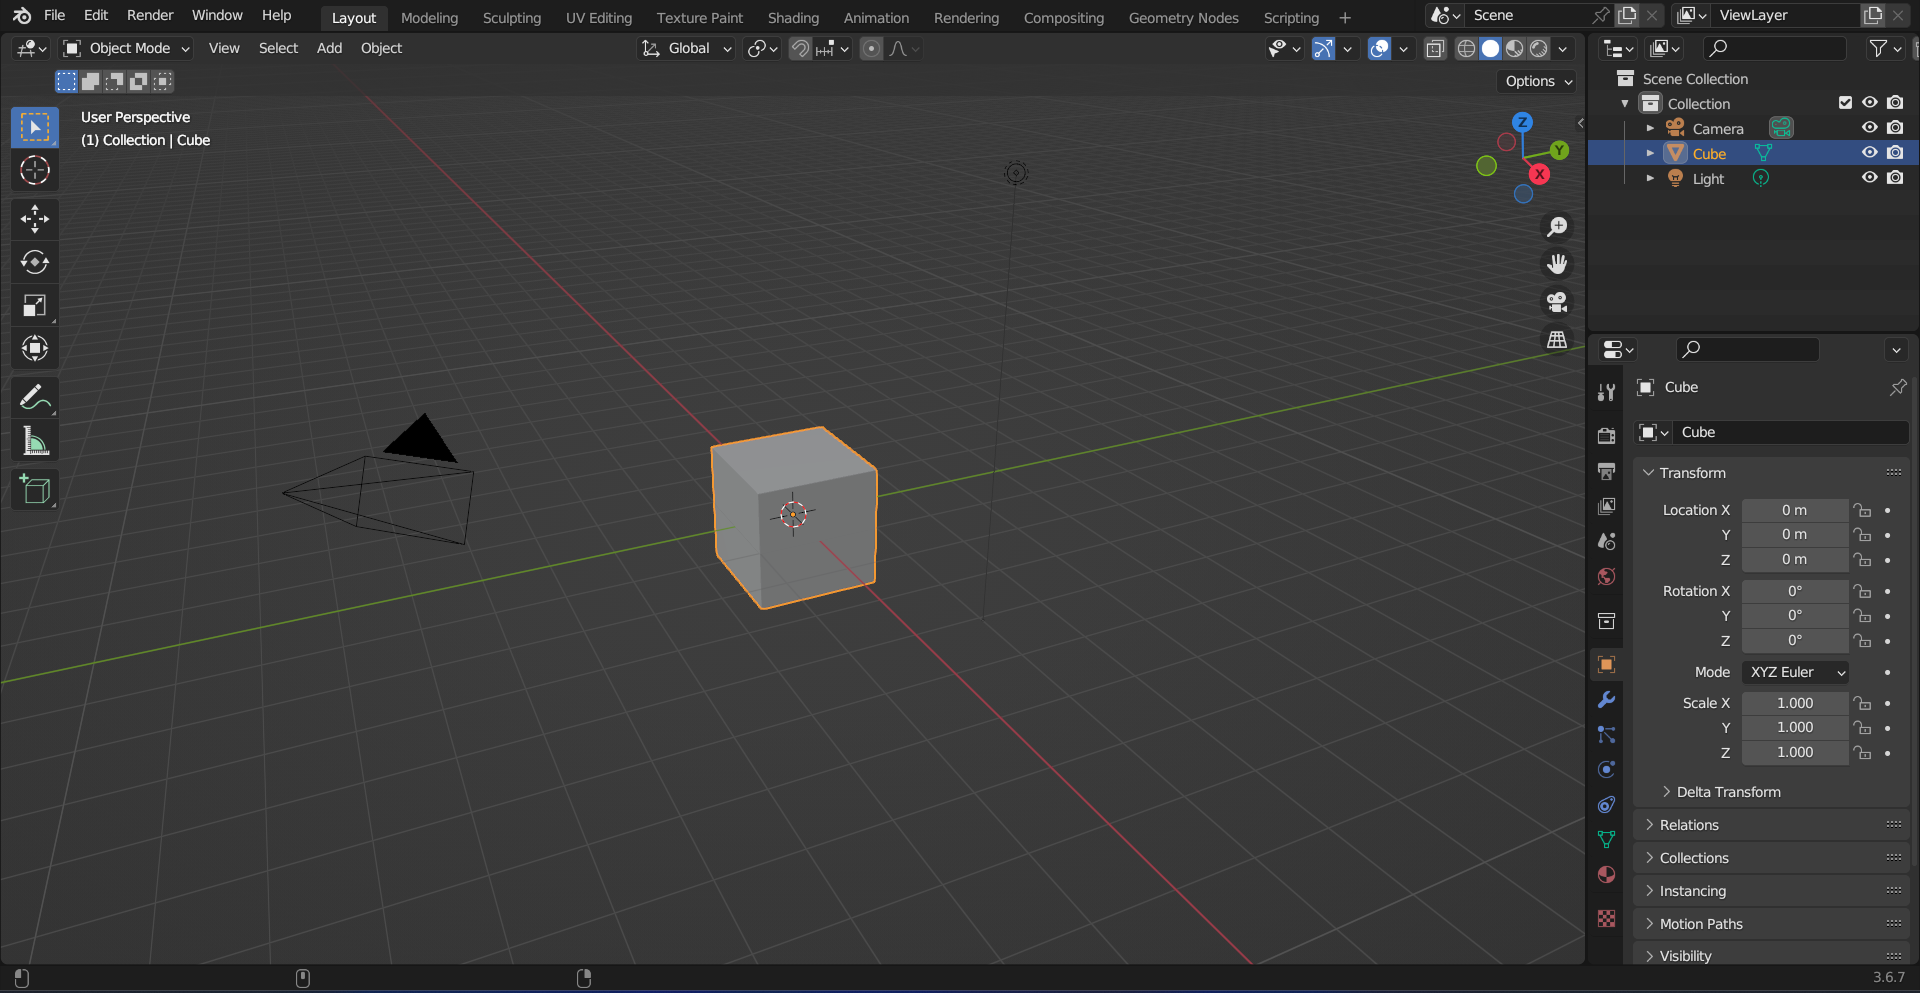
\includegraphics[width=1\textwidth]{images/defaultobjectmode.png}
\caption{Standard Ansicht im Object Mode}
\label{fig:defaultobjectmode}
\end{figure}

\item \textbf{Edit Mode:} Ist ein Modus für das Editieren einer Objektform mit verschiedensten Werkzeugen. Man kann die
einzelnen Vertices \footnote{Blender \cite{Vertices}}, Kanten und Flächen auf Basis von verschiedenen Kontrollpunkten bearbeiten.
\begin{figure}[h]
\centering
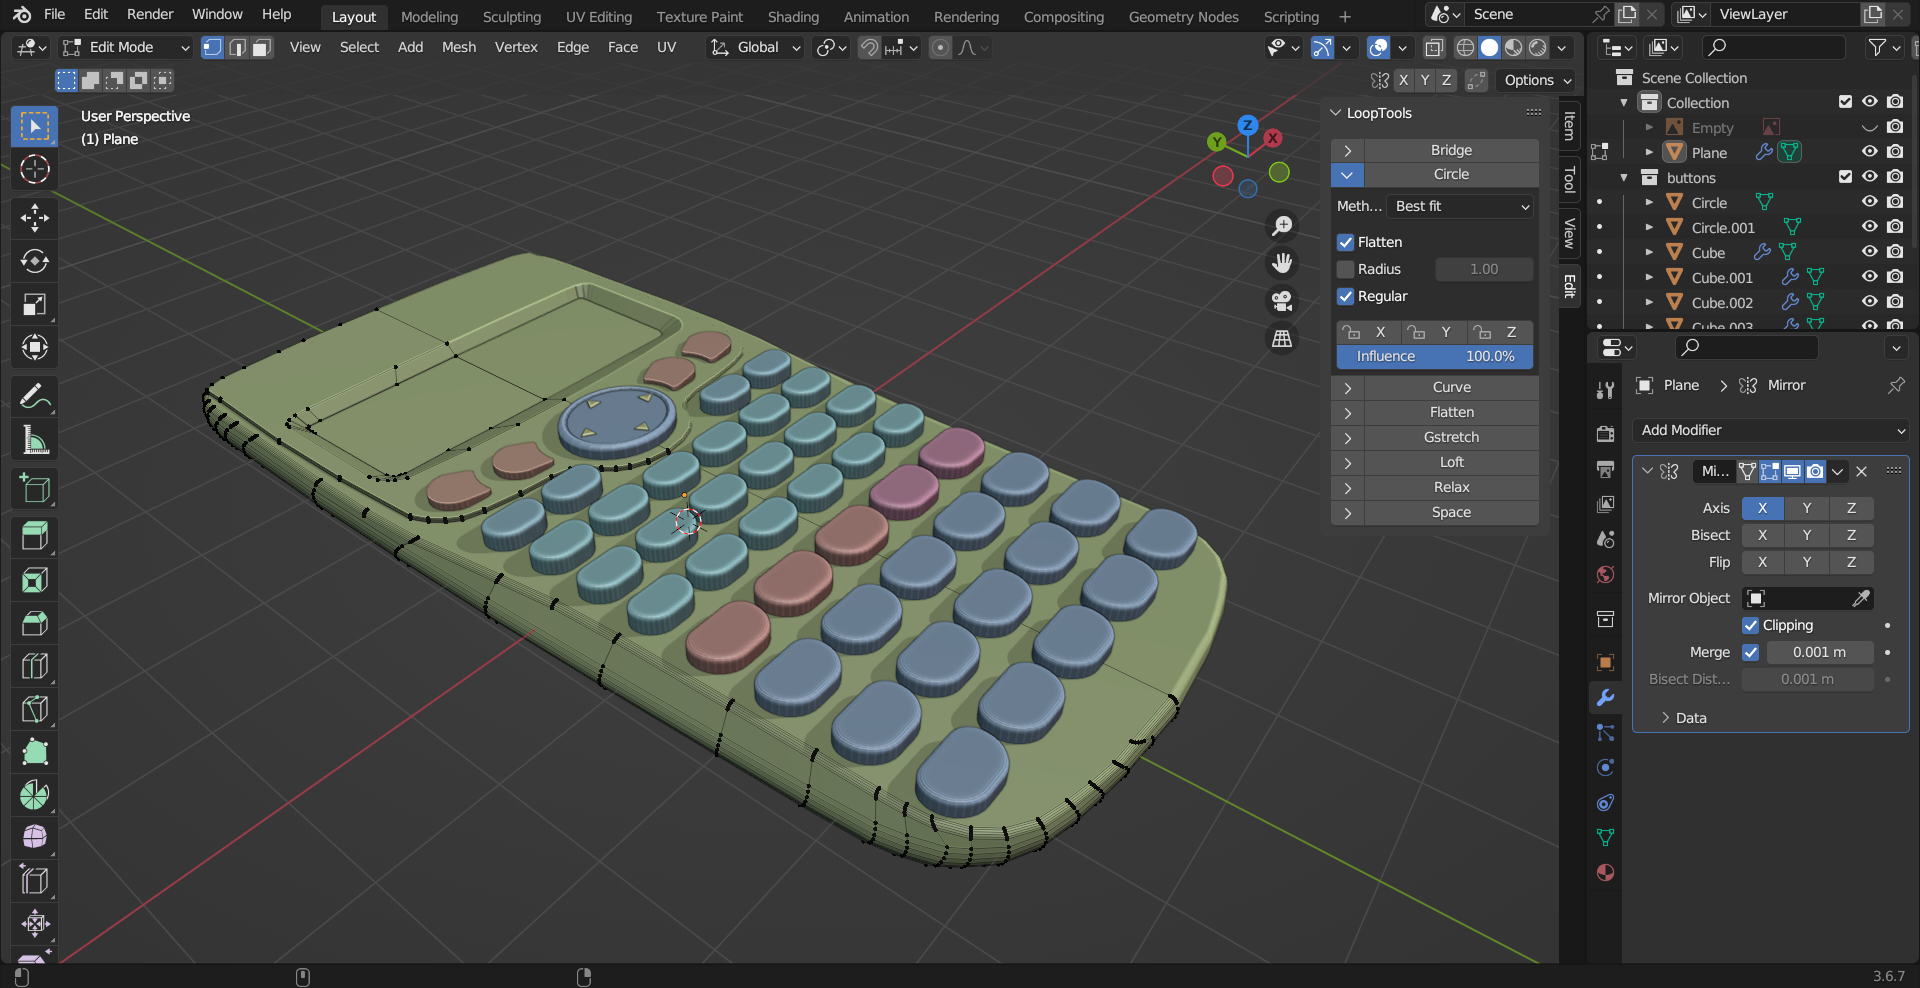
\includegraphics[width=1\textwidth]{images/calculatoreditmode.png}
\caption{Edit Mode Ansicht auf das Calculator Objekt}
\label{fig:calculatoreditmode}
\end{figure}

\item \textbf{Texture Paint Mode:} Ein Mesh-Only \footnote{Blender \cite{Mesh}} Modus der es dir ermöglicht Texturen direkt auf das Model im 3D-Viewport
zu zeichnen.
\begin{figure}[h]
\centering
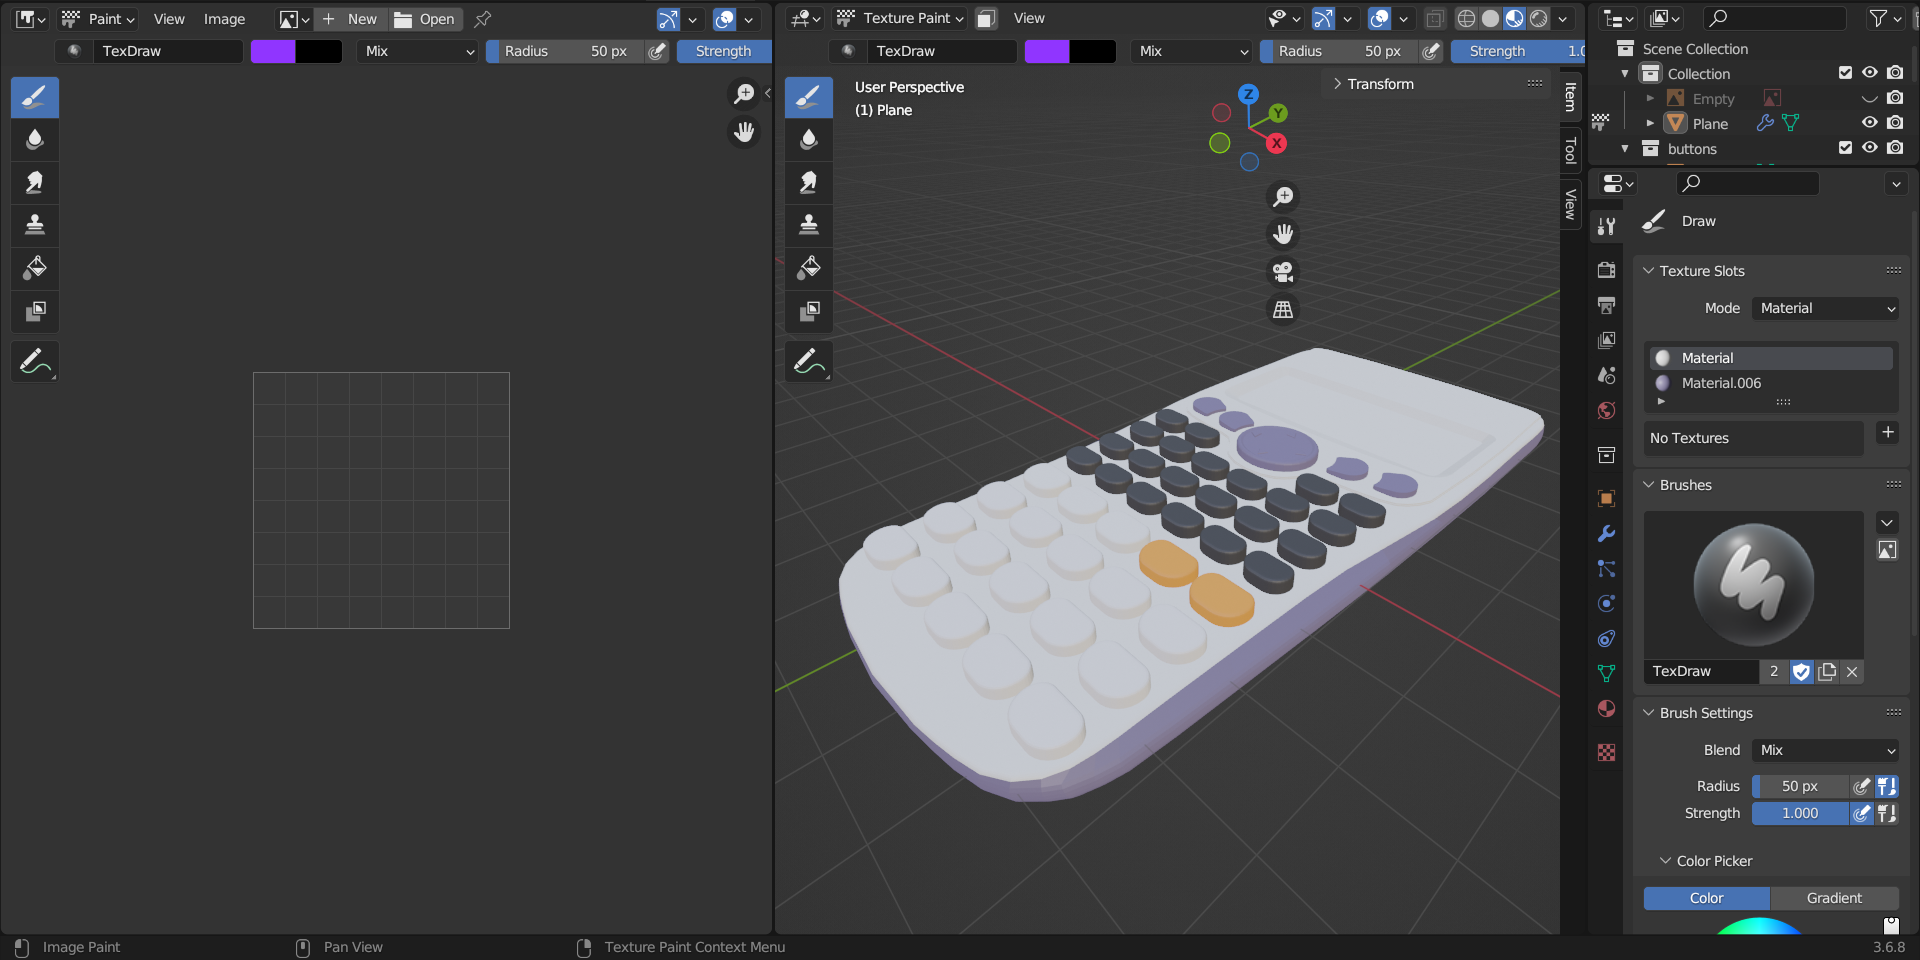
\includegraphics[width=1\textwidth]{images/texturepaintmode.png}
\caption{Standard Ansicht im Texture Paint Mode}
\label{fig:texturepaintmode}
\end{figure}
\end{itemize}

\subsection{Blender - Hierarchie}
Im folgenden Abschnitt wird erklärt, wie Blender aufgebaut ist und wie die einzelnen verwendeten Werkzeuge und Modifier
\footnote{Blender \cite{Modifier}} funktionieren. Es wurden einige Modelle erstellt, aber für ein einfacheres Verständnis
wurde für alle Beispielbilder das Taschenrechner-Modell verwendet.
\begin{figure}[h]
\centering
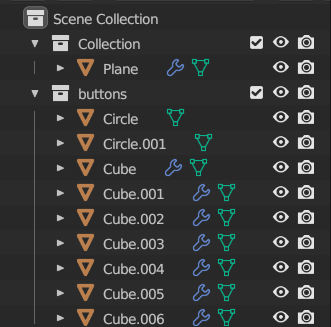
\includegraphics[width=0.8\textwidth]{images/blenderhierarchy.png}
\caption{Ansicht auf die Hierarchie des Taschenrechner Modells}
\label{fig:blenderhierarchy}
\end{figure}

In dieser Abbildung ist die Hierarchie und der Inhalt des Hauptmenüs zu sehen. Wie zu sehen ist, besteht die Szene aus
vielen wichtigen Komponenten die zusammenspielen, um die gewünschte Funktion zu erzielen. Darunter sind folgende Objekte:

\begin{itemize}
\item \textbf{Scene Collection:} Die umfassende Collection enthält das gesamte Modell mit allen Teilen. Collections
werden mehrmals in der Abbildung verwendet, um die Hierarchie besser zu strukturieren. Sie haben jedoch keinen Einfluss
auf das Objekt selbst.
\item \textbf{Plane:} Das Mesh dient zur groben Formgebung des Taschenrechners.
\item \textbf{Circles/Cubes:} Die Circles und Cubes sind die einzelnen Buttons.
\end{itemize}

In der Abbildung ist zu erkennen, dass einige Formen mit einem blauen/grünen Zeichen markiert sind.
Das blaue Zeichen kennzeichnet einen Modifier, das heißt, das Objekt hat einen oder mehrere Modifier.
Das grüne Zeichen steht für Data Properties und zeigt an, dass sich diese verändert haben.

\subsubsection{Blender - Modifier}
Im vorherigen Abschnitt wurden erwähnt das Modifier verwendet werden. Modifier ermöglichen verschiedene zusätzliche
Funktionen an einem Objekt.

\begin{figure}[h]
\centering
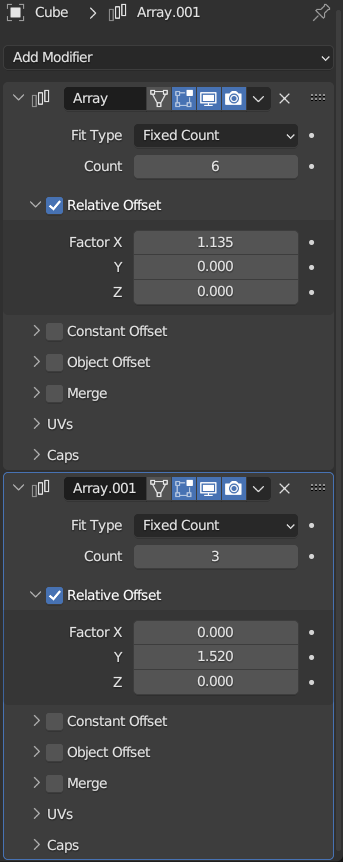
\includegraphics[width=0.8\textwidth]{images/blendermodifier.png}
\caption{Darstellung des benutzen Modifier im Taschenrechnermodell}
\label{fig:blendermodifier}
\end{figure}

In der Abbildung ist der Array Modifier zweimal zu sehen. Dieser wurde verwendet, um nicht jeden Knopf des Taschenrechners
einzeln modellieren zu müssen, sondern nur einen bestimmten Knopf horizontal oder vertikal mit beliebiger Versetzung zu
kopieren. Dabei haben die einzelnen Zeilen verschiedene Funktionen.
\begin{itemize}
\item \textbf{Fit Type:} Es besteht die Möglichkeit, entweder eine feste Anzahl von Objektkopien auszuwählen oder eine
Länge anzugeben, die dem Array entspricht.
\item \textbf{Count:} In dem Feld rechts daneben steht die Anzahl, wie oft das Objekt kopiert werden soll.
\item \textbf{Relative Offset:} Die relative Verschiebung basiert immer auf dem zuvor kopierten Modell und hat drei
Faktoren, die jeweils eine der drei Koordinaten darstellen. In diesem Fall soll es um 1.520 auf der x-Achse nach rechts
verschoben werden.
\end{itemize}

\section{Menü}
Die Implementierung des UI/UX-Systems erfolgt über das Menü. Aufgrund einer umfassenden Recherche über verschiedene
Menüarten wurde die Wahl für die Realisierung eines NearMenus getroffen. Dabei handelt es sich um eine frei
bewegliche Menüleiste, die sich auf Hüfthöhe des Benutzers befindet und synchron mit dessen Bewegungen mitfließt.

Das Ziel ist es, das Menü so einfach wie möglich zu gestalten und trotzdem alle notwendigen Funktionen zu integrieren.
\begin{figure}[h]
\centering
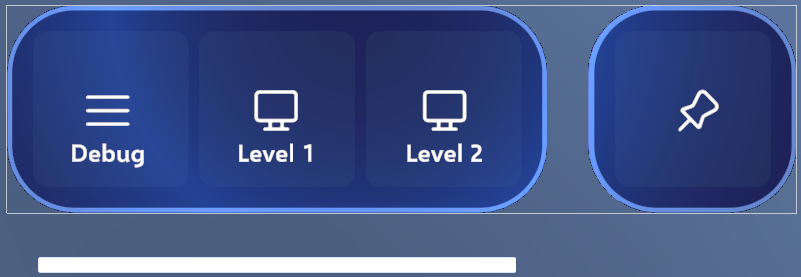
\includegraphics[width=0.8\textwidth]{images/menubar.png}
\caption{Darstellung des Hauptmenüs ohne Debugmenü im Unity Editor}
\label{fig:menübar}
\end{figure}

\subsection{Menü-Hierarchie}
In dem folgendem Abschnitt wird darauf eingegangen wie das Menü im Unity Editor aufgebaut ist und wie die einzelnen
Buttons Grundsätzlich funktionieren.

\begin{figure}[h]
\centering
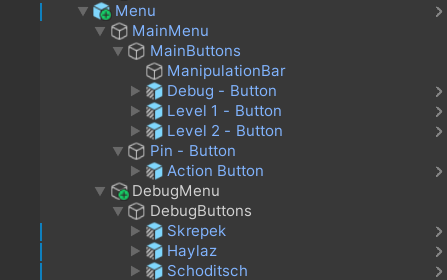
\includegraphics[width=0.8\textwidth]{images/menuHierarchy.png}
\caption{Hauptmenühierarchie im Unity Editor}
\label{fig:menühierarchy}
\end{figure}


In dieser Abbildung ist die Hierarchie und der Inhalt des Hauptmenüs zu sehen. Wie zu sehen ist, besteht die Szene aus
vielen wichtigen Komponenten die zusammenspielen, um die gewünschte Funktion zu erzielen. Darunter sind folgende Objekte:

\begin{itemize}
\item \textbf{Menü:} Das Prefab, dem alle einzenen Buttons etc. zugewiesen sind.
\item \textbf{ManipulationBar:} Ist ein GameObject, dem das \textit{ObjectManipulator.cs} Skript zugewiesen ist, welches
die händische Menüführung ermöglicht.
\item \textbf{Debug-Button:} Der Debug-Button ist ausschließlich für das Entwicklerteam vorgesehen. Beim Aktivieren öffnet
sich ein erweitertes Menü oberhalb des Hauptmenüs, das zusätzliche Funktionen für das Bugfixing während des Betriebs
bereitstellt.
\begin{figure}[h]
\centering

\includegraphics[width=0.8\textwidth]{images/debugmenubar.png}
\caption{Darstellung des Debug Menüs im Unity Editor}
\label{fig:debugmenübar}
\end{figure}
\item \textbf{Skrepek:} Das Prefab ist ein Button der für Skrepek vorbereitet ist, um mögliche Skripts für Bugfixing
während des Betriebes einzubringen.
\item \textbf{Haylaz:} Das Prefab ist ein Button der für Haylaz vorbereitet ist, um mögliche Skripts für Bugfixing
während des Betriebes einzubringen.
\item \textbf{Schoditsch:} Das Prefab ist ein Button der für Schoditsch vorbereitet ist, um mögliche Skripts für Bugfixing
während des Betriebes einzubringen.
\item \textbf{Level 1/2-Button:} Diese Prefabs stellen die Buttons für das Level wechseln da, ihnen ist das
\textit{SceneChange.cs} Skript zugewiesen.
\item \textbf{Pin-Button:} Der Pin-Button ermöglicht das Fixieren des Menüs an einer geeigneten Stelle. Dies ist besonders nützlich,
wenn der Benutzer sich an einen Tisch setzt und das Menü entsprechend positionieren möchte. Die
Positionierung erfolgt mithilfe der ManipulationsBar.
\end{itemize}

\subsection{Laden der Level}
Im vorherigen Abschnitt wurde bereits die grobe Funktionalität der Buttons erklärt. Das Drücken eines der Level-Buttons
(Level 1, Level 2) löst das \textit{SceneChange.cs} Skript aus.Dieser Code ist für die Änderung der aktuellen Szene
verantwortlich. Die zu ladende Szene wird durch die Variable sceneToLoad definiert, die in Unity festgelegt wird und das
gewünschte Level angibt.

\begin{lstlisting}[style=csharp, caption=Auf Knopfdruck Szene wechseln.]
using UnityEngine;
using UnityEngine.SceneManagement;
public class SceneChanger : MonoBehaviour
{
public string sceneToLoad;

// Assign this method to the button's onClick event in the Unity Editor.
public void ChangeScene()
{
SceneManager.LoadScene(sceneToLoad);
Debug.Log("Button clicked. Loading scene: " + sceneToLoad);
}
}
\end{lstlisting}

\begin{figure}[h]
\centering
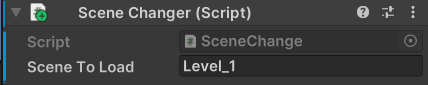
\includegraphics[width=0.8\textwidth]{images/sceneToLoad.png}
\caption{Darstellung der SceneToLoad Variable, anhand des Level_1 Buttons.}
\label{fig:scenetoload}
\end{figure}

\subsection{UI/UX}
Im folgenden Abschnitt werden die Ziele genannt, auf die sich bei der Menüerstellung konzentriert wurde.
\begin{itemize}
\item \textbf{Blickzentrierung und Interaktionsmodelle:}
Die Menüleiste bewegt sich auf Hüfthöhe mit dem Benutzer mit und ermöglicht so eine natürliche und intuitive Interaktion.
Der Benutzer kann die Bedienelemente einfach durch Blickkontakt auswählen, was die Benutzerfreundlichkeit erhöht und die
Bedienung der Anwendung erleichtert.
\item \textbf{Konsistenz im Design:}
Die klare Gestaltung der Buttons mit aussagekräftigen Symbolen trägt zur Konsistenz und Benutzerfreundlichkeit bei.
Eine einheitliche visuelle Sprache erleichtert es dem Benutzer, die Funktionen der Buttons zu verstehen, selbst wenn er
sie zum ersten Mal verwendet.
\item \textbf{Kontextsensitive Funktionen:}
Der Debug-Button bietet erweiterte Funktionen, die speziell für Entwickler relevant sind. Diese kontextsensitiven
Optionen sind wichtig für die Fehlersuche und tragen dazu bei, die Entwicklungszeit zu optimieren. Gleichzeitig bleibt
die Benutzeroberfläche für den Endbenutzer sauber und übersichtlich.
\item \textbf{Anpassungsmöglichkeiten für den Benutzer:}
Die Option, das Menü mit dem Pin-Button zu fixieren und mit der Grab-Bar frei zu bewegen, gibt dem Benutzer die
Kontrolle über die Positionierung des Menüs. Diese Anpassungsmöglichkeiten tragen dazu bei, die Anwendung an
verschiedene Nutzerszenarien anzupassen und die individuellen Bedürfnisse der Benutzer zu berücksichtigen.
Feedback und Animationen
\end{itemize}

\section{Ping Level}
In diesem Level wird das IT-Grundprinzip eines Pings zwischen zweier
PCs dargestellt. Das Kabel zwischen den zwei PCs wird von der
HoloLens getracked und mittels Kurvenberechnung wird dann eine
unsichtbare Kurve über dieses Kabel gezeichnet. Wenn dann der Benutzer
auf die Enter Taste auf einem PC drückt wird ein Ping-Paket simuliert
und auf dieser Kurve von einem PC zu dem anderen geschickt.

\subsection{Object Tracking}
Durch verwendung von bereitgestellten Technologien der HoloLens2
werden die zwei PCs und das Kabel getracked.
%Hier dann noch code zum Object Tracking einfügen

\subsection{Kurvenberechnung}
Durch Berechnung der Kurve wird das Kabel als Kurve gespeichert
und dadurch wird es ermöglicht, dass das 3D-Ping-Paket über diese
Kurve von einem PC zum anderen läuft.
%Hier dann noch code zur Kurvenberechnung einfügen

\section{Knapsack Problem Level}
Im zweiten Level dieses Projekts steht das Knapsack-Problem im Fokus.
Ziel ist es, diesen Programmieralgorithmus mithilfe von Augmented Reality
(AR) visuell darzustellen. Dieser Algorithmus wird nicht nur in der Höheren
Technischen Lehranstalt (HTL) vermittelt, sondern die Benutzer sollen
ihn auch selbst programmieren können.

Der Level beginnt damit, dass der Benutzer aufgefordert wird, auf eine
horizontale, flache Oberfläche zu schauen. Diese Oberfläche kann ein Tisch,
der Boden oder ähnliches sein. Der Benutzer wird dann gebeten, für eine bestimmte
vorgegebene Zeit auf diese Oberfläche zu schauen. Nach Ablauf der vorgeschriebenen
Zeit wird dann das Inventar als auch das \textit{infoObjekt} platziert.

Das Inventar wird durch ein 3x3 zweidimensionales Gitter repräsentiert, ähnlich
wie das Inventar in einem Spiel. Zusätzlich befinden sich auf der Oberfläche 11 Bauklötze,
die mit QR-Codes versehen sind. Diese Bauklötze repräsentieren die Items, die der Benutzer
in das Inventar legen kann. Durch Aufheben und Nahheranhalten an die HoloLens wird der QR-Code gescannt.
Dadurch werden das dazugehörige 3D-Modell, der Wert, Gewicht und der Name des Items angezeigt.
Diese Informationen sind für den Benutzer wichtig, um das Gewicht des Items und
seinen Einfluss auf das Inventar zu verstehen.

Wenn der Bauklotz erfolgreich platziert wurde, wird automatisch der Knapsack-Algorithmus für die perfekte Lösung,
und die Berechnung des eigenen Inventars gestartet um stets den aktuellen Wert zu sehen.

Insgesamt bietet dieses Unity Level für die HoloLens 2 eine interaktive und visuelle Erfahrung,
bei der die Benutzer das Knapsack-Problem nicht nur verstehen, sondern auch praktisch anwenden können.

\subsection{Knapsack-Problem Level Hirarchie}
In dem folgendem Abschnitt wird darauf eingegangen wie eine Szene in dem Unity Editor aufgebaut ist und wie diese Grundsätzlich
funktionieren.\\

\begin{figure}[h]
    \centering
    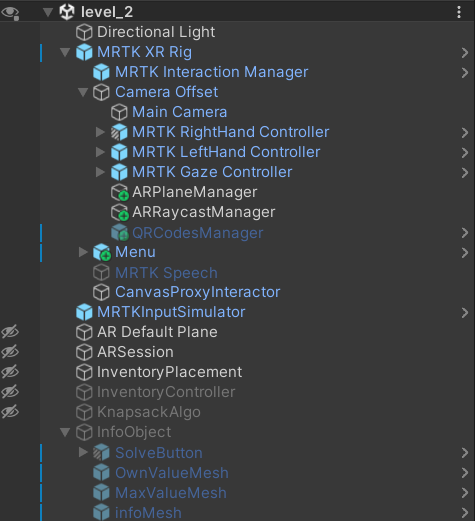
\includegraphics[scale=0.8]{images/Level2Hirarchy}
    \caption{Knapsack-Problem Levels Hirarchie Unity Editor.}
    \label{fig:level2_hierarchy}
\end{figure}

In dieser Abbildung ist die Hirarchie und der Inhalt des Knapsack-Problem Levels / Szene\footnote{Unity \cite{Scene}} 2 zu sehen.
Wie zu sehen ist, besteht die Szene aus vielen wichtigen Komponenten die zusammenspielen, um das gewünschte Ergebnis
zu erzielen. Darunter sind folgende Objekte:

\begin{itemize}
    \item \textbf{level-2:} Die Scene in der Alle Unity-Game-Objekte enthalten sind.
    \item \textbf{AR Default Plane:} In der Augmented Reality (AR)-Entwicklung bezieht sich ein Plane\footnote{Unity \cite{Plane}} normalerweise
    auf eine erkannte horizontale Fläche in der realen Welt, auf der virtuelle Objekte platziert werden können. Diese
    Flächen können zum Beispiel Tische, Böden oder andere ebene Oberflächen sein. Das Erkennen und Tracking von Planes
    ist entscheidend, um AR-Objekte realistisch in die Umgebung zu integrieren.
    \item \textbf{ARSession:} In Unity und AR Foundation bezieht sich die "ARSession" im Allgemeinen auf die
    Hauptkomponente, die die AR-Funktionalitäten steuert und koordiniert.
    \item \textbf{InventoryPlacement:} Ist ein Game Objekt, dem das \textit{Knapsackscript.cs} Script zugewiesen ist und
    bei Szenen-Start aktiv ist. Dieses Game Objekt kümmert sich darum, dass das Inventar richtig in der Augmented Reality
    Welt platziert wird.
    \item \textbf{InventoryController:} Das Game Objekt, dem das \textit{InventorryController.cs} Script zugewiesen ist
    und nach Abschluss des InventoryPlacement Scripts aktiviert wird. Dieses Objekt ist die Hauptschnittstelle
    zwischen den QR-Codes und dem 3D Inventar Modell und kümmert sich darum neue QR-Codes innerhalb des Modells zu erkennen
    und zu verspeichern.
    \item \textbf{KnapsackAlgo:} GameObjekt, dem das \textit{KnapsackAlgo.cs} Script zugewiesen ist und bei platzieren
    eines QR-Codes innerhalb des Inventars auslöst, den maximalen erreichbaren Wert, die perfekte Lösung und den Wert des
    selbst erstellten Inventars berechnet.
    \item \textbf{bestSolutionPrefab:} Dieses Objekt ist das Prefab\footnote{Unity \cite{Prefab}} für die Perfekte Lösung.
    Diesem Objekt ist das 3D Modell des Inventars untergeordnet und diesem Inventar sind Prefabs für QRCodes untergeordnet.
    In jeder Zelle des Inventars ist ein eigenes QRCode Prefab um anschließend die berechnete perfekte Lösung darstellen zu können.
    Diesem Objekt ist das \textit{PerfectSolutionVisualizer.cs} Script zugewiesen, dass sich darum kümmert die perfekte Lösung
    anzuzeigen.
    \begin{figure}[h]
        \centering
        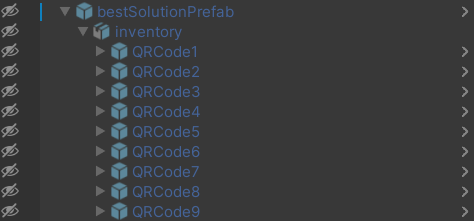
\includegraphics[scale=0.8]{images/bestSolPref}
        \caption{bestSolutionPrefab Objekt Hirarchie.}
        \label{fig:bestSolutionPrefab_hirarchie}
    \end{figure}
    \item \textbf{InfoObject:} Dieses Game Objekt ist eine Sammlung aus mehreren Unity Game Objekten. Dieses Objekt wird bei platzieren
    des Inventars neben dem Inventar mitplatziert. Bei den Objekten handelt es sich hierbei um den \textit{BestSolutionButton},
    der bei Knopfdruck einer der mehreren besten Lösungen visuell veranschaulicht, und drei \textit{TextMeshes}, um die
    berechneten Werte, und auch Informationen anzuzeigen.
    Zusätzlich ist hier zusehen, dass diese 4 Objekte dem \textit{infoObject} untergeordnet sind, was bedeutet, dass diese Objekte
    \textit{children} von dem \textit{infoObejct} sind. Das übergeordnete OBjekt wird hier dann als \textit{parent} bezeichnet.
\end{itemize}

In der Abbildung ist zu sehen, dass ein Paar Game Objekte ausgegraut und nicht ausgegraut sind und, dass neben ein paar Game Objekten ein durchgestrichenes Auge zu sehen ist.
Wenn ein Game Objekt im Unity Editor ausgegraut ist bedeutet das, dass dieses GameObjekt und somit alle angehängiten Scripts von diesem Game Objekt deaktiviert sind.
Das bedeutet, dass dieses Game Objekt samt allen Scripts zu Szenenbeginn nicht aufgerufen und somit auch nicht ausgeführt werden. Nicht ausgegraute Game Objekte widerum sind
daher genau das Gegenteil. Das beudetet, dass das Game Objekt selbst samt allen angehängiten Scripts alle aktiviert sind und somit zu Szenenbeginn aufgerufen und ausgeführt werden.

Wenn neben einem Game Objekt das durchgestrichene Auge zu sehen ist bedeutet das nur, dass dieses Game Objekt im Unity Editor nicht zu sehen ist. Andererseits, wenn kein Zeichen
neben dem Game Objekt zu sehen ist, ist dieses Objekt im Unity Editor sichtbar. Dies dient dazu, dass falls in der Unity Szene viele Game Objekte vorhanden sind, dass man
diejenige ausblendet die nicht im Editor sichtbar sein müssen wie zum Beispiel Tesh Meshes oder Lables.

\subsection{Verwendung von QR-Codes}
Im vorangegangenen Abschnitt wurde bereits darauf hingewiesen, dass QR-Codes in diesem Level verwendet werden,
um die verschiedenen Items zu repräsentieren. Diese QR-Codes spielen eine entscheidende Rolle, indem sie dazu dienen,
vielfältige Informationen zu den einzelnen Objekten zu speichern und sie anschließend in einer virtuellen Umgebung
abzubilden. Im folgenden Abschnitt möchten wir näher darauf eingehen, wie genau diese QR-Codes generiert werden
und welchen Zweck sie innerhalb der Augmented Reality (AR)-Applikation erfüllen. Hierbei wird insbesondere betrachtet,
wie die Generierung der Codes erfolgt und auf welche Weise sie innerhalb der Anwendung zur Interaktion mit den realen Objekten verwendet werden.

\subsubsection{Inhalt der QR-Codes}
Die Informationen, die in einem QR-Code gespeichert werden, sind begrenzt. In unserem Anwendungsfall wird lediglich eine
einzelne Zahl im Bereich von 1 bis 11 abgespeichert. Diese Zahlen repräsentieren die 11 verschiedenen Modelle, die wir
unterscheiden möchten. Da nur eine Zahl gespeichert wird, genügt ein QR-Code der Größe 21x21 Module (Version 1). Die
geringe Anzahl von Modulen ermöglicht eine schnellere Erkennung auch über größere Distanzen.
%TODO: Testen und Grafik erstellen um zu zeigen das es eine Rolle spielt welche version wir verwenden + wie groß die sind

Die zugehörigen Zahlen erhalten in der Software, genauer gesagt in der Klasse \textit{QRItem.cs}, einen Kontext. Der folgende Codeausschnitt zeigt dies:

\begin{lstlisting}[style=csharp, caption={}, label=code:update]
public class QRItem
{
    public struct QRData
    {
        public int id;
        public string name;
        public Vector3 position;
        public int weight;
        public int value;
    }

    public QRData qrData;

    public Dictionary<int, QRData> items = new Dictionary<int, QRData>()
    {
        {1, new QRData { id = 1, name = "Laptop", weight = 70, value = 100 }},
        {2, new QRData { id = 2, name = "Router", weight = 25, value = 50 }},
        {3, new QRData { id = 3, name = "Maus", weight = 20, value = 30 }},
        // ...
        {11, new QRData { id = 11, name = "Handy", weight = 30, value = 100 }}
    };

    public QRItem(int id)
    {
        items.TryGetValue(id, out qrData);
    }
}
\end{lstlisting}

In dieser Klasse wird ein Dictionary verwendet, das den Zahlen die folgenden Informationen zuordnet:

\begin{itemize}
    \item \textbf{Item Id:} Die numerische Kennung im QR-Code.
    \item \textbf{Item Name:} Die Bezeichnung des Items, das dieser QR-Code repräsentiert.
    \item \textbf{Item Position:} Die Position des Items in der virtuellen Umgebung.
    \item \textbf{Item Weight:} Das Gewicht des Items.
    \item \textbf{Item Value:} Der Wert des Items.
\end{itemize}

Diese Informationen spielen eine wesentliche Rolle in der weiteren Berechnung des Knapsack-Algorithmus.

\subsubsection{QR-Code Tracking}
Das Tracking der QR-Codes erfolgt mithilfe des \textit{QRCodeManager.cs} Skripts. Dieses Klasse ist ein Singleton, das
die Erkennung und Verfolgung der QR-Codes steuert.
Das folgende UML-Diagramm zeigt die wichtigsten Methoden und zusammenhängenden Klassen:
%TODO: Abbildung einfügen
Nach der Erkennung eines QR-Codes erfolgen eine Reihe von Schritten, um diese Informationen zu speichern, verarbeiten
und zuletzt darzustellen.
Hier eine kurze Übersicht:
%TODO: Übersicht einfügen

\subsection{Inventory Placement Game Objekt}
Um eine präzise Interaktion zwischen der realen und augmentierten Realität zu gewährleisten, ist der Zugriff auf die
Kamera erforderlich, um die physische Umgebung zu erfassen. Durch die Analyse der erfassten Daten können Ebenen
identifiziert werden, die entscheidend sind, um eine genaue Platzierung von Inventargegenständen zu erreichen.

In diesem Abschnitt wird das \textit{Inventory Placement} Game Objekt mit dem angehängten \textit{AnchorScript.cs}
behandelt. Dieses Script enthält die \textbf{PlacedObjectOnLookedAtDesk} Klasse, welche alle Funktionen für das Berechnen
der Position und Platzierung des Inventars beinhaltet. Diese Funktionen werden in den nächsten Abschnitten detailliert erläutert.

\begin{figure}[h]
    \centering
    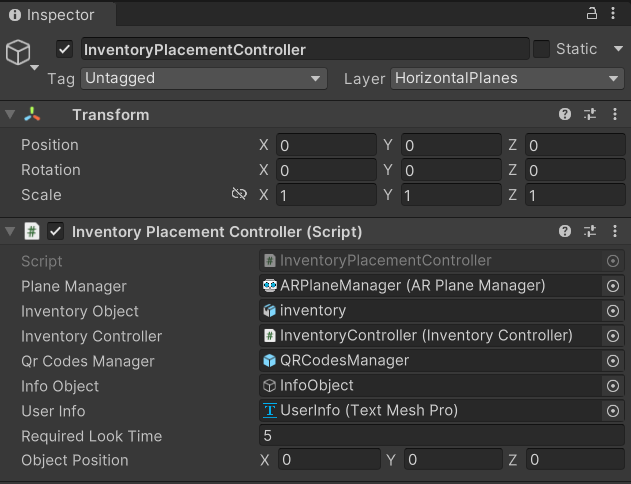
\includegraphics[scale=0.8]{images/invPlace_Editor}
    \caption{inventoryPlacement Objekt im Editor}
    \label{fig:inventoryPlacement_Editor}
\end{figure}

Die Abbildung \ref{fig:inventoryPlacement_Editor} zeigt das \textit{inventoryPlacement}-Objekt im Unity Editor. Hier
können verschiedene Einstellungen vorgenommen werden, darunter die Ebene, in der dieses Objekt liegt, die Koordinaten
im Unity Editor und die angehängte Komponente \textit{AnchorScript.cs}. Zudem sind vordefinierte Werte für bestimmte
Variablen sichtbar. Diese Variablen umfassen:

\begin{itemize}
    \item \textbf{Raycast Manager:} Das Game Objekt des ARRaycastManagers aus der Level 2 Szene.
    \item \textbf{Plane Manager:} Das Game Objekt des ARPlanesManagers aus der Level 2 Szene.
    \item \textbf{Inventory Object:} Das 3D-Modell des Inventars aus dem Prefab Ordner.
    \item \textbf{Inventory Controller:} Das Script des InventoryControllers.
    \item \textbf{QR Codes Manager:} Das Game Objekt des QRCodeManagers aus der Level 2 Szene.
    \item \textbf{Info Object:} Das Game Objekt des Info-Objekts aus der Level 2 Szene.
    \item \textbf{Required Look Time:} Die vorgeschriebene Zeit, die der Benutzer auf ein Plane schauen muss, damit das
    Inventar platziert wird.
\end{itemize}

Im Unity Editor können die Werte dieser Variablen direkt verändert werden, was Auswirkungen auf die Ausführung des Codes hat.\\

\subsubsection{Klassenvariablen}
\begin{lstlisting}[style=csharp, caption={Klassenvariablen der PlacedObjectOnLookedAtDesk Klasse}, label=code:anchor_var]
public ARRaycastManager raycastManager;
public ARPlaneManager planeManager;
public GameObject inventoryObject;
public InventoryController inventoryController;
public GameObject qrCodesManager;
public GameObject infoObject;
public float requiredLookTime = 5.0f;
public Vector3 objectPosition;

private ARPlane selectedDeskPlane;
private float lookStartTime = -1f;
private bool objectPlaced = false;
private float heightOffset = 0.001f;

private bool canStartScript = false;
\end{lstlisting}

Die gezeigten Klassenvariablen in Codeabschnitt \ref{code:anchor_var} sind Teil der \textit{PlaceObjectOnLookedAtDesk} Klasse. Öffentliche
(\textbf{public}) Variablen repräsentieren Objekte und Werte, die im Unity Editor festgelegt und übergeben werden. Dies
ermöglicht einen direkten Zugriff auf diese Objekte im Code. Die Vektor-Variable \textit{objectPosition} spielt eine
entscheidende Rolle für die präzise Platzierung der perfekten Lösung. Die privaten (\textbf{private}) Variablen dienen
der lokalen Speicherung von Werten, die von keiner anderen Klasse benötigt werden.

\subsubsection{Startverzögerung}
\begin{lstlisting}[style=csharp, caption={Beginn des Anchor Scripts}, label=code:Start]
void Start()
{
    StartCoroutine(DelayedStart());
}
\end{lstlisting}
Zu Beginn des Levels für das "Knapsack-Problem" wird die Lebenszyklusmethode \textit{Start()} aufgerufen. Diese Funktion
startet dann die Coroutine \textbf{DelayedStart()}. Die Startverzögerung wird hier verwendet, um dem \textit{ARPlaneManager}
ausreichend Zeit zu geben, um Ebenen in der Umgebung des Benutzers zu scannen und zu markieren. Dies ist von Bedeutung,
um eine solide Grundlage für die spätere präzise Platzierung des Inventars zu gewährleisten.\\

\begin{lstlisting}[style=csharp, caption={Verzoegerter Start}, label=code:DelayedStart]
private IEnumerator DelayedStart()
{
    yield return new WaitForSeconds(3.0f);
    canStartScript = true;
}
\end{lstlisting}
In der Funktion \textbf{DelayedStart()} wird eine Verzögerung von 3 Sekunden durchgeführt, bevor \textit{canStartScript}
auf true gesetzt wird. Diese Verzögerung ermöglicht es dem \textit{ARPlaneManager}, ungestört die Umgebung zu scannen.
Die Aktivierung von \textit{canStartScript} markiert den Zeitpunkt, ab dem die \textit{Update()} Methode ihre Ausführung
fortsetzen kann. Dieser gestaffelte Startprozess gewährleistet eine reibungslose Erfassung von AR-Planes und legt somit
einen soliden Grundstein für die präzise Platzierung von Inventargegenständen in der augmentierten Realität.

\subsubsection{Frame-Aktualisierung zur Identifikation des gewünschten AR-Planes}
Da in der Umgebung mehrere AR-Planes gescannt und markiert werden, ist es notwendig, ständig zu aktualisieren, welcher
der markierten und gescannten Planes tatsächlich das beabsichtigte ist. Um dieses Verhalten zu erreichen, wird die
Lebenszyklusmethode \textit{Update()} verwendet. Diese Methode sorgt dafür, dass stets der gewünschte AR-Plane
ausgewählt ist. Falls der Benutzer seinen Blick auf einen anderen, näher gelegenen Plane richtet, wird dieser als der
neue ausgewählte Plane betrachtet.\\

\begin{lstlisting}[style=csharp, caption={Update Funktion}, label=code:Update]
void Update()
{
    if (!objectPlaced && canStartScript)
    {
        List<ARRaycastHit> hits = new List<ARRaycastHit>();
        % Use Camera.main.transform.forward as the ray direction
        if (raycastManager.Raycast(new Ray(Camera.main.transform.position, Camera.main.transform.forward), hits, TrackableType.Planes))
        {
            ARPlane closestPlane = FindClosestPlane(hits);
            if (closestPlane != null)
            {
                if (selectedDeskPlane == null || selectedDeskPlane != closestPlane)
                {
                    selectedDeskPlane = closestPlane;
                    lookStartTime = Time.time; % Start the timer when a new plane is selected.
                }
                float timeLookedAtPlane = Time.time - lookStartTime;
                if (timeLookedAtPlane >= requiredLookTime)
                {
                    PlaceObjectOnDesk(selectedDeskPlane);
                    objectPlaced = true;
                }
            }
            else
            {
                selectedDeskPlane = null;
            }
        }
        else
        {
            selectedDeskPlane = null;
        }
    }
}
\end{lstlisting}
Die \textit{Update()} Methode bildet das Herzstück des AR-Anker-Skripts, das die kontinuierliche Interaktion zwischen
der realen und augmentierten Realität orchestriert. Der Ablauf beginnt mit einer sorgfältigen Prüfung, ob das
Inventarobjekt noch nicht platziert wurde (\textit{!objectPlaced}) und ob das Skript gestartet werden kann
(\textit{canStartScript}). Diese Bedingungen dienen dazu sicherzustellen, dass der Platzierungsprozess nur startet,
wenn die Voraussetzungen erfüllt sind.\\

\begin{lstlisting}[style=csharp, caption={Raycasting}, label=code:Raycasting]
List<ARRaycastHit> hits = new List<ARRaycastHit>();
if (raycastManager.Raycast(new Ray(Camera.main.transform.position, Camera.main.transform.forward), hits, TrackableType.Planes))
{
    % Weitere Verarbeitung der Treffer...
}
\end{lstlisting}
Sobald die Startbedingungen erfüllt sind, wird ein Raycasting durchgeführt, um die AR-Planes in der Umgebung zu
identifizieren. Der Richtungsvektor des Rays wird durch \textit{Camera.main.transform.forward} bestimmt.\\

\begin{lstlisting}[style=csharp, caption={Kürzest entfernte Plane}, label=code:FindClosestPlane]
ARPlane closestPlane = FindClosestPlane(hits);
\end{lstlisting}
Der nächste Schritt beinhaltet die Bestimmung des am kürzesten entfernten AR-Planes durch Aufruf der Funktion
\textbf{FindClosestPlane(hits)}. Diese Funktion vergleicht die Distanzen aller getroffenen AR-Planes und gibt den
nächstgelegenen zurück.\\

\begin{lstlisting}[style=csharp, caption={Plane auswählen und timer starten}, label=code:TimeMeasurement]
if (selectedDeskPlane == null || selectedDeskPlane != closestPlane)
{
    selectedDeskPlane = closestPlane;
    lookStartTime = Time.time; % Starten des Timers, wenn ein neues Plane ausgewählt wird.
}
\end{lstlisting}
Die ausgewählten AR-Plane werden daraufhin miteinander verglichen, und wenn ein neues AR-Plane ausgewählt wird oder der
aktuelle AR-Plane sich geändert hat, wird die Zeitmessung (\textit{lookStartTime}) gestartet. Diese Zeitmessung erfasst
die Dauer, für die der Benutzer auf den aktuellen AR-Plane blickt.\\

\begin{lstlisting}[style=csharp, caption={Blickzeit messen}, label=code:TimeUpdate]
float timeLookedAtPlane = Time.time - lookStartTime;
\end{lstlisting}
Die gemessene Blickzeit (\textit{timeLookedAtPlane}) wird in jedem Frame aktualisiert, indem die aktuelle verstrichene
Zeit seit dem Start des Blicks auf den AR-Plane gemessen wird.\\

\begin{lstlisting}[style=csharp, caption={Platzier-Funktion aufrufen}, label=code:Placement]
if (timeLookedAtPlane >= requiredLookTime)
{
    PlaceObjectOnDesk(selectedDeskPlane);
    objectPlaced = true;
}
\end{lstlisting}
Wenn die gemessene Blickzeit die erforderliche Blickzeit überschreitet, wird die Funktion
\textbf{PlaceObjectOnDesk(selectedDeskPlane)} aufgerufen, um das Inventarobjekt auf dem ausgewählten AR-Plane zu
platzieren. Zusätzlich wird \textit{objectPlaced} auf true gesetzt, um zu signalisieren, dass das Objekt platziert
wurde und weitere Überprüfungen gestoppt werden sollen.\\

\begin{lstlisting}[style=csharp, caption={Plane null setzen}, label=code:NoPlaneHit]
else
{
    selectedDeskPlane = null;
}
\end{lstlisting}
Falls kein AR-Plane getroffen wurde, wird \textit{selectedDeskPlane} auf null gesetzt, um sicherzustellen, dass keine
vorherigen Auswahlinformationen beibehalten werden.\\

Dieser Ablauf setzt sich in jedem Frame fort, bis die vorgegebene Blickzeit erreicht ist und somit das Inventarobjekt
erfolgreich auf dem AR-Plane platziert wurde.\\

\subsubsection{Das am kürzesten entfernte Plane finden}
\begin{lstlisting}[style=csharp, caption={Kürzest entfernte Plane - Funktion}, label=code:findclosestplane]
ARPlane FindClosestPlane(List<ARRaycastHit> hits)
{
    ARPlane closestPlane = null;
    float closestDistance = float.MaxValue;
    foreach (var hit in hits)
    {
        ARPlane plane = planeManager.GetPlane(hit.trackableId);
        if (plane != null)
        {
            float distanceToPlane = Vector3.Distance(Camera.main.transform.position, hit.pose.position);
            if (distanceToPlane < closestDistance)
            {
                closestPlane = plane;
                closestDistance = distanceToPlane;
            }
        }
    }
    return closestPlane;
}
\end{lstlisting}
Die Funktion \textit{FindClosestPlane} durchläuft eine Liste von \textit{ARRaycastHit}-Objekten, die durch den
Raycasting-Prozess erstellt wurden. Für jedes Trefferobjekt wird der zugehörige AR-Plane über den \textit{planeManager} abgerufen.
Dann wird die Entfernung von der Kameraposition zum Trefferpunkt des Rays auf dem AR-Plane berechnet.

Die Schleife sucht nach dem am nächsten gelegenen AR-Plane, indem sie die Distanz für jeden Treffer vergleicht.
Das am nächsten gelegene AR-Plane (\textit{closestPlane}) und die entsprechende Distanz (\textit{closestDistance})
werden aktualisiert, wenn ein näherer Treffer gefunden wird. Am Ende wird das am nächsten gelegene AR-Plane zurückgegeben.

Diese Funktion wird in der Regel in AR-Anwendungen verwendet, um das AR-Plane zu identifizieren, auf das der Benutzer am
längsten schaut, bevor eine Aktion ausgeführt wird.\\

\textbf{Beispiel}:
Angenommen, es existieren drei AR-Planes in der Umgebung des Benutzers und die Liste \textit{hits} enthält folgende
Trefferpunkte:
\begin{itemize}
    \item 1. Trefferpunkt auf Plane A: Entfernung = 2 Meter
    \item 2. Trefferpunkt auf Plane B: Entfernung = 1 Meter
    \item 3. Trefferpunkt auf Plane C: Entfernung = 3 Meter
\end{itemize}
Während des Durchlaufs durch die Trefferpunkte würde die Funktion \textit{FindClosestPlane} in diesem Beispiel das
AR-Plane B zurückgeben, da es die kürzeste Distanz von 1 Meter zur Kameraposition hat.\\

\subsubsection{Berechnung der Position und Aktivierung/Deaktivierung sämtlicher Objekte}
\begin{lstlisting}[style=csharp, caption={Inventar platzier - Funktion}, label=code:placeobject]
void PlaceObjectOnDesk(ARPlane deskPlane)
{
    qrCodesManager.SetActive(true);
    Vector3 objectPosition = deskPlane.center + Vector3.up * heightOffset;
    Quaternion objectRotation = Quaternion.Euler(-90f, 0f, 0f);
    GameObject instantiatedObject = Instantiate(inventoryObject, objectPosition, objectRotation);
    instantiatedObject.transform.localScale = new Vector3(20f, 20f, 20f);
    Vector3 infoObjectPosition = objectPosition - Vector3.forward * 4.415f + Vector3.right * 0.4f;
    infoObject.transform.position = infoObjectPosition;
    infoObject.SetActive(true);
    inventoryController.SetInventoryObject(instantiatedObject);
    inventoryController.gameObject.SetActive(true);
    planeManager.planePrefab.SetActive(false);
    gameObject.SetActive(false);
}
\end{lstlisting}
Diese Funktion übernimmt mehrere wichtige Aufgaben im Kontext der Augented Reality-Anwendung die den sicheren weiteren
Ablauf der Appplikation versichert.

\begin{enumerate}
    \item \textbf{Aktivierung des QR-Code Managers:} Die Funktion startet damit, den QR-Code Manager zu aktivieren,
    was das Tracken von QR-Codes ermöglicht.
    \item \textbf{Berechnung der Objektposition und Rotation:} Anschließend wird die Position des Inventar-Objekts
    berechnet. Dazu wird die Flächenmitte des ausgewählten AR-Planes genutzt, und die Rotation des Objekts wird auf
    der x-Achse festgelegt.
    \item \textbf{Instantiierung des Objekts:} Das Inventar-Objekt wird dann durch die Verwendung der
    \textbf{Instantiate}-Funktion erstellt und auf eine bestimmte Größe skaliert.
    \item \textbf{Platzierung des Info-Objects:} Die Position des Info-Objects, das aus TextMeshes und Buttons besteht,
    wird ebenfalls berechnet und aktiviert, um für den Benutzer sichtbar zu sein.
    \item \textbf{Setzen des Inventar-Objekts im InventoryController:} Das platzierte Inventar-Objekt wird an den
    \textit{InventoryController} weitergeleitet und dort als aktuelles Inventarobjekt festgelegt um sicherzustellen,
    dass hier dann in Folge auf das selbe Objekt zugegriffen wird.
    \item \textbf{Aktivierung des InventoryControllers:} Nach der erfolgreichen Platzierung des Inventar-Objekts und
    Aktivierung des Info-Objects wird der \textit{InventoryController} aktiviert, um die Inventarverwaltung zu starten.
    \item \textbf{Sichtbarkeit der Planes ausschalten:} Da die AR-Planes nach erfolgreicher Platzierung der Objekte nicht
    mehr sichtbar sein sollen, weil sie nichtmehr gebraucht werden, werden sie mit
    \textit{planeManager.planePrefab.SetActive(false)} deaktiviert.
    \item \textbf{Deaktivierung des Skripts:} Schließlich wird das \textit{AnchorScript.cs} deaktiviert, um weitere
    ressourcenintensive Aktualisierungen zu stoppen.
\end{enumerate}\\

Dieser Ablauf stellt sicher, dass nach der Erkennung und Auswahl eines AR-Planes das Inventar-Objekt präzise platziert
wird und alle notwendigen Elemente aktiviert bzw. deaktiviert werden, um eine nahtlose Integration von realer und
augmentierter Realität zu gewährleisten.

\subsection{Inventory Controller Game Objekt}
Das \textit{Inventory Controller} Game Objekt spielt eine entscheidende Rolle bei der Überwachung und Verwaltung des
Inventars in der Augmented Reality (AR)-Anwendung. Durch das angehängte \textit{InventoryController.cs} Script wird die
\textbf{InventoryController} Klasse realisiert. Diese Klasse ist verantwortlich für die Erkennung neuer Gegenstände im
Inventar, die Überprüfung auf verfügbaren Platz im Inventar, die Berechnung der Zellenposition anhand der QR-Code-Koordinaten
und die Speicherung der Positionen dieser Items in einem \textit{2D Array}.

Der Zugriff auf die Begrenzungen (\textit{Bounds}) des Inventarmodells ermöglicht es, ständig zu überwachen, ob der
Benutzer ein neues Element in das Inventar gelegt hat. Dieser Ansatz gewährleistet eine präzise Kontrolle über die
Platzierung von Gegenständen im Inventar.

Das \textit{InventoryController.cs} Script interagiert dabei aktiv mit den AR-Elementen, insbesondere den QR-Codes, um
den Platzbedarf der Gegenstände zu überwachen und ihre Positionen im Inventar festzulegen. Zusätzlich interagiert der
\textit{InventoryController} auch mit dem \textit{KnapsackAlgo} Game Objekt, in dem es das verspeicherte \textit{2D Array}
immer weitergibt um damit rechnen zu können.\\

\begin{figure}[h]
    \centering
    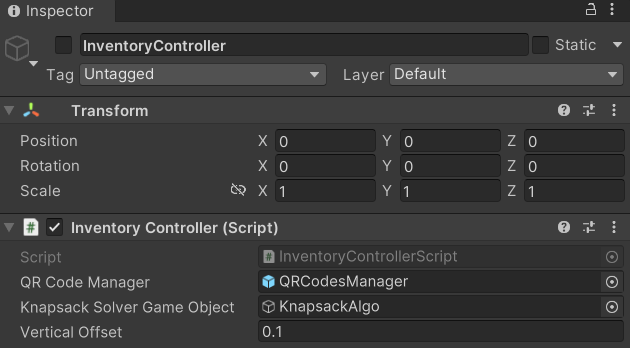
\includegraphics[scale=0.8]{images/invCon_Editor}
    \caption{IventoryController Objekt im Editor}
    \label{fig:InventoryController_Editor}
\end{figure}

Die Abbildung \ref{fig:InventoryController_Editor} zeigt das \textit{iventoryController}-Objekt im Unity Editor.  Hier
können verschiedene Einstellungen vorgenommen werden, darunter die Ebene, in der dieses Objekt liegt, die Koordinaten
im Unity Editor und die angehängte Komponente \textit{InventoryController.cs}. Zudem sind vordefinierte Werte für bestimmte
Variablen sichtbar. Diese Variablen umfassen:

\begin{itemize}
    \item \textbf{QRCodesManager:} Das QRCodesManager Game Objekt aus der Level 2 Szene.
    \item \textbf{Knapsack Solver Game Objekt:} Das KnapsackAlgo Game Objekt aus der Level 2 Szene.
    \item \textbf{Vertical Offset:} Float Wert um den die Bounds\footnote{Unity \cite{Bounds}} des Inventory Objekts auf der X-Achso erweitert werden.\\
\end{itemize}

\subsubsection{InventoryController Klassenvariablen}
\begin{lstlisting}[style=csharp, caption={Klassenvariablen der InventoryController Klasse}, label=code:controller_var]
void PlaceObjectOnDesk(ARPlane deskPlane)
{
    public GameObject QRCodeManager;
    public GameObject knapsackSolverGameObject;

    private SortedDictionary<System.Guid, GameObject> activeQRObjects;

    private GameObject inventoryObject;
    public float verticalOffset = 0.1f;
    private Bounds inventoryBounds;
    private int numRows = 3;
    private int numColumns = 3;
    private int[,] idGrid;
    private KnapsackScript knapsackScript;
    private int cap;
    private int currWeight = 0;
    private string message;
    private HashSet<int> processedItems;
}
\end{lstlisting}
Die gezeigten Klassenvariablen in Codeabschnitt \ref{code:controller_var} sind Teil des \textit{InventoryController} Klasse.
Öffentliche(\textbf{public}) Variablen repräsentieren Objekte und Werte, die im Unity Editor festgelegt und übergeben werden. Dies
ermöglicht einen direkten Zugriff auf diese Objekte im Code. Die float-Variable \textit{verticalOffset} spielt hier eine
wichtige Rolle, für die erweiterung der \textit{Bounds} von dem Inventar Modell. Die privaten (\textbf{private}) Variablen dienen
der lokalen Speicherung von Werten, die von keiner anderen Klasse benötigt werden.\\

\subsubsection{Start des InventoryControllers}
\begin{lstlisting}[style=csharp, caption={Start Funktion des InventoryControllers}, label=code:controller_start]
void Start()
{
    activeQRObjects = QRCodeManager.GetComponent<QRCodesVisualizer>().qrCodesObjectsList;
    knapsackScript = knapsackSolverGameObject.GetComponent<KnapsackScript>();
    cap = knapsackScript.capacity;
    processedItems = new HashSet<int>();
    UpdateInventoryBounds();
    InitializeIDGrid();
}
\end{lstlisting}
Die \textbf{Start()} Funktion wird zu Beginn des Inventory Controllers aufgerufen und aufgeführt. Hier werden die
wichtigen Objekte die für den weiteren Verlauf des Programms notwendig sind deklariert beziehungsweise erstellt und
ebenfalls werden die beiden Funktionen \textbf{UpdateInventoryBounds()} und \textbf{InitializeIDGRid()} aufgerufen.\\

\subsubsection{Neue Bounds setzen}
\begin{lstlisting}[style=csharp, caption={Funktion um Inventar Bounds zu erweitern}, label=code:controller_updateBounds]
private void UpdateInventoryBounds()
{
    if (inventoryObject != null)
    {
        Bounds localBounds = GetBounds(inventoryObject);
        ExtendBounds(ref localBounds, verticalOffset);
        inventoryBounds = localBounds;
    }
}
\end{lstlisting}
Um zu erreichen, dass man ein Item wirklich in die Bounds des Inventars legen kann wird in der \textbf{UpdateInventoryBounds()}
Funktion genau dies ausgeführt. Es werden die aktuellen Bounds des Inventars gespeichert und diese werden dann mittels
der \textbf{ExtendBounds()} Funktion erweitert und anschließend werden diese Bounds als neue Bounds gespeichert.\\

\subsubsection{Bounds des Inventars ermitteln}
\begin{lstlisting}[style=csharp, caption={Funktion um Bounds zu ermitteln}, label=code:controller_getBounds]
private Bounds GetBounds(GameObject obj)
{
    Renderer renderer = obj.GetComponent<Renderer>();
    return renderer != null ? renderer.bounds : new Bounds(obj.transform.position, Vector3.one);
}
\end{lstlisting}
Die von \ref{code:controller_updateBounds} aufgerufene Funktion \textbf{GetBounds} greift auf den Renderer\footnote{Unity \cite{Renderer}}
des Inventar Modells zu um dadurch auf die Bounds zuzugreifen zu können, denn der Renderer ist dafür verantwortlich,
dass das Modell überhaupt sichtbar ist. Wenn dieser Renderer ungleich \textbf{null} ist, gibt er die neuenn Bounds zurück und speichert
sie in \textit{localBounds} von Codeabschnitt \ref{code:controller_updateBounds}.\\

\subsubsection{Inventory Bounds erweitern}
\begin{lstlisting}[style=csharp, caption={Funktion um Bounds zu erweitern}, label=code:controller_extendBounds]
private void ExtendBounds(ref Bounds bounds, float offset)
{
    bounds.center = new Vector3(bounds.center.x, bounds.center.y + offset / 2, bounds.center.z);
    bounds.extents = new Vector3(bounds.extents.x, bounds.extents.y + offset / 2, bounds.extents.z);
}
\end{lstlisting}
Um anschließend diese Bounds zu erweitern um zu erkennen ob QR-Koordinaten innerhalb von diesen Bounds ist wird die von
\ref{code:controller_updateBounds} aufgerufene Funktion \textbf{ExtendBounds()} ausgeführt. Diese Funktion erzielt, dass die
Bounds von dem Inventar Modell auf der X-Achso um das \textit{Vertical Offset} erweitert werden. Nach Abschluss dieser Funktion
sehen die Bounds von diesem Modell dann folgendermaßen aus:
\begin{figure}[h]
    \centering
    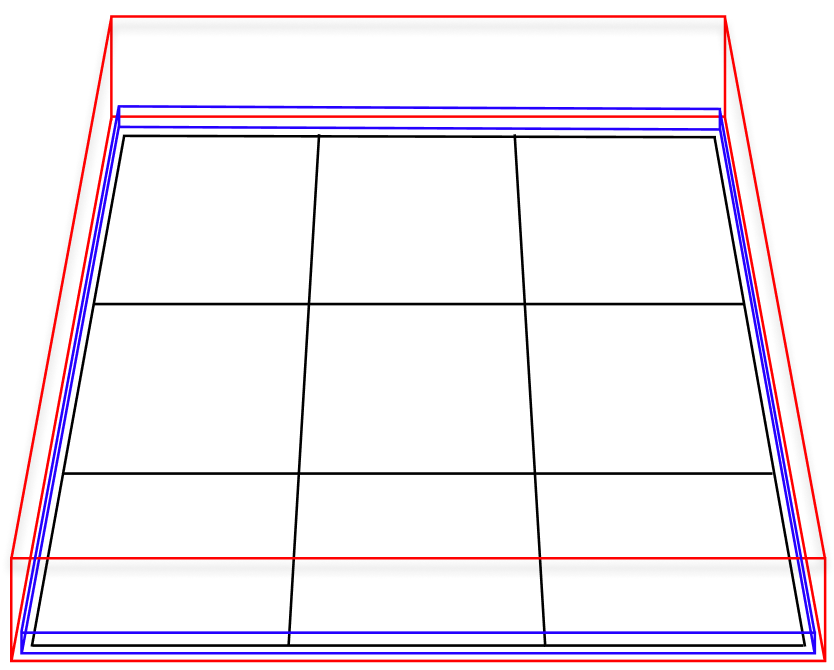
\includegraphics[scale=0.4]{images/extendedBounds}
    \caption{Erweiterte Bounds des Inventar Modells}
    \label{fig:extended_inventoryBounds}
\end{figure}

Auf der Abbildung \ref{fig:extended_inventoryBounds} ist eine einfache schematische Zeichnung des zweidimensionalen Inventars zu sehen. Die
blaue Umrandung repräsentiert die Begrenzungen (Bounds) vor der Ausführung der Funktion \textbf{UpdateInventoryBounds()}
aus dem Codeabschnitt \ref{code:controller_updateBounds}. Nachdem die Funktion ausgeführt wurde, wird die rote Umrandung
dargestellt. Durch die neuen Bounds wird deutlich, dass insbesondere die Begrenzung entlang der X-Achse erweitert wurde.

Die Erweiterung der Bounds ist von entscheidender Bedeutung, da nicht erweiterte Bounds die Höhe der Bauklötze nicht
berücksichtigen würden. Dies könnte dazu führen, dass ein QR-Code, der sich tatsächlich innerhalb der Bounds befindet,
als außerhalb betrachtet wird, wenn die Höhe der Bauklötze nicht angemessen einbezogen wird.

Diese Anpassungen sind wichtig, um sicherzustellen, dass die Begrenzungen des Inventars korrekt erfasst werden und somit
eine präzise Verortung von QR-Codes innerhalb der Augmented-Reality-Anwendung gewährleistet ist.\\

\subsubsection{ID Grid Initialisierung}
\begin{lstlisting}[style=csharp, caption={Initialisierung des idGrids}, label=code:controller_initialize]
private void InitializeIDGrid()
{
    idGrid = new int[numRows, numColumns];
}
\end{lstlisting}
Die in Codeabschnitt \ref{code:controller_start} aufgerufene Funktion initialisiert das idGrid mit \textit{numRows} und
\textit{numColumns} also wird das idGrid als \textit{int [3,3]} initialisiert.\\

\subsubsection{Update Funktion}
\begin{lstlisting}[style=csharp, caption={Initialisierung des idGrids}, label=code:controller_update]
void Update()
{
    UpdateGrid();
}
\end{lstlisting}
Nach Abschluss des Codes aus Codeabschnitt \ref{code:controller_start} wird anschließend die \textit{Lebenszyklusmethode}
\textbf{Update()} ausgeführt. Diese Funktion ruft jeden Frame die \textbf{UpdateGrid()} Funktion auf, auf die im nächsten
Abschnitt genau eingegangen wird.\\

\subsubsection{Funktion für neue Items innerhalb des Bounds}
\begin{lstlisting}[style=csharp, caption={Code fuer ueberpruefen neuer Items im Inventar}, label=code:controller_check]
void UpdateGrid()
{
    lock (activeQRObjects)
    {
        foreach (var item in activeQRObjects.Values)
        {
            QRCode qRCode = item.GetComponent<QRCode>();
            Vector3 worldPosition = item.transform.TransformPoint(qRCode.item.qrData.position);

            if (item != null && inventoryBounds.Contains(worldPosition))
            {
                int itemId = qRCode.item.qrData.id;

                if (!processedItems.Contains(itemId))
                {
                    if (currWeight + qRCode.item.qrData.weight <= cap)
                    {
                        processedItems.Add(itemId);
                        message = " ";
                        Vector2 startGridPosition = CalculateGridPosition(worldPosition);
                        idGrid[(int)startGridPosition.x, (int)startGridPosition.y] = itemId;
                        knapsackScript?.UpdateInfoMesh(message);
                        currWeight += qRCode.item.qrData.weight;
                        EventManager.GridUpdate(idGrid);
                    }
                    else
                    {
                        message = "Item hat zu viel Gewicht!";
                        knapsackScript?.UpdateInfoMesh(message);
                    }
                }
            }
            else if (!inventoryBounds.Contains(worldPosition) && processedItems.Contains(qRCode.item.qrData.id) && ContainsId(qRCode.item.qrData.id))
            {
                int itemId = qRCode.item.qrData.id;
                processedItems.Remove(itemId);
                RemoveItem(itemId);
                currWeight -= qRCode.item.qrData.weight;
                EventManager.GridUpdate(idGrid);
            }
        }
        PrintGrid();
    }
}
\end{lstlisting}
Die vorliegende Funktion, \texttt{UpdateGrid()}, ist maßgeblich für die Überwachung und Verwaltung von neu hinzugefügten
oder entfernten Items im Inventar verantwortlich. Zu Beginn eines jeden Frames wird das \texttt{activeQRObjects}-Dictionary
gesperrt, um Thread-Sicherheit zu gewährleisten. Anschließend erfolgt eine Iteration durch jedes Element in diesem Dictionary
mittels einer \texttt{foreach}-Schleife.\\

Innerhalb dieser Schleife wird für jedes Objekt die zugehörige \texttt{QRCode}-Komponente extrahiert, und die Weltposition
des Objekts wird durch Transformation der lokalen Position des QR-Codes unter Berücksichtigung der Transformation des
übergeordneten Objekts berechnet.\\

Die Hauptüberprüfung erfolgt daraufhin, ob das aktuelle Item nicht null ist und ob seine Weltposition innerhalb der durch
\texttt{inventoryBounds} definierten Grenzen liegt. Wenn diese Bedingungen erfüllt sind, wird das Item als "hinzugefügt"
betrachtet.\\

Im weiteren Verlauf wird überprüft, ob die ID des Items bereits in der Menge der verarbeiteten Items (\texttt{processedItems})
vorhanden ist. Falls nicht, wird überprüft, ob das Hinzufügen des Items das aktuelle Gesamtgewicht (\texttt{currWeight})
zusammen mit dem Gewicht des Items unter die maximale Kapazität (\texttt{cap}) bringt.\\

Wenn diese Bedingungen erfüllt sind, wird das Item in die Menge der verarbeiteten Items aufgenommen, eine Nachricht wird
auf Leer gesetzt, und die Position des Items im zweidimensionalen Array \texttt{idGrid} wird aktualisiert. Zusätzlich
wird die Anzeige des Inventars durch den Aufruf der Methode \texttt{UpdateInfoMesh} des \texttt{knapsackScript}
aktualisiert, und das aktuelle Gewicht des Inventars wird entsprechend angepasst. Schließlich wird ein Ereignis
(\texttt{GridUpdate}) ausgelöst, um andere Teile des Systems über die Aktualisierung des Grids zu informieren.
\begin{figure}[h]
    \centering
    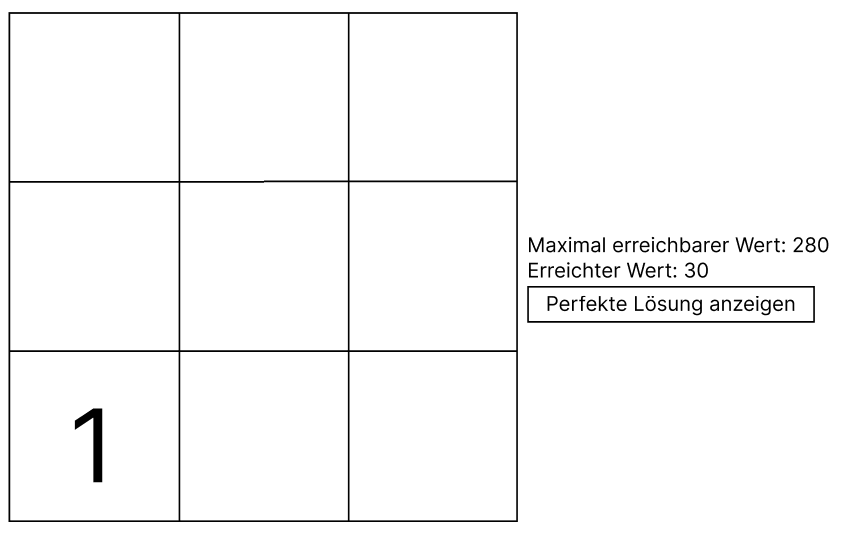
\includegraphics[scale=0.6]{images/itemAdded}
    \caption{Item zu Inventar hinzugefügt}
    \label{fig:controller_itemAdded}
\end{figure}

In Abbildung \ref{fig:controller_itemAdded} ist der Zustand nach dem Hinzufügen eines Items dargestellt. In Zelle 7 wurde
das Item mit der \textit{ID: 1} hinzugefügt. Nach dem Hinzufügen des Items wird der \textit{Knapsack Algorithmus} ausgelöst
und anschließend die beiden TextMehes aktualisiert, indem in dem oberen TextMesh der maximal erreichbare Wert angezeigt wird
und in dem unteren der Wert des selbst zusammengestellten Inventars.\\

Nachdem das Item im Inventar platziert wurde sieht nun dass \textit{idGrid} folgendermaßen aus:
\begin{lstlisting}[style=csharp, caption={ID verspeichert}, label=code:controller_savedID]
int idGrid = [[0, 0, 0],
              [0, 0, 0],
              [1, 0, 0]];
\end{lstlisting}\\

Das Hashset \textit{processedItems} sieht nach platzieren des Items dann so aus:
\begin{lstlisting}[style=csharp, caption={ID verspeichert}, label=code:controller_savedID]
processedItems = [1];
\end{lstlisting}\\

Sollte das Gewicht des hinzugefügten Items die Kapazität überschreiten, wird eine Fehlermeldung generiert, und die
Aktualisierung des Grids wird unterbunden. Die Fehlermeldung und der resultierende Zustand des Grids sind in Abbildung
\ref{fig:controller_itemToHeavy} dargestellt.
\begin{figure}[h]
    \centering
    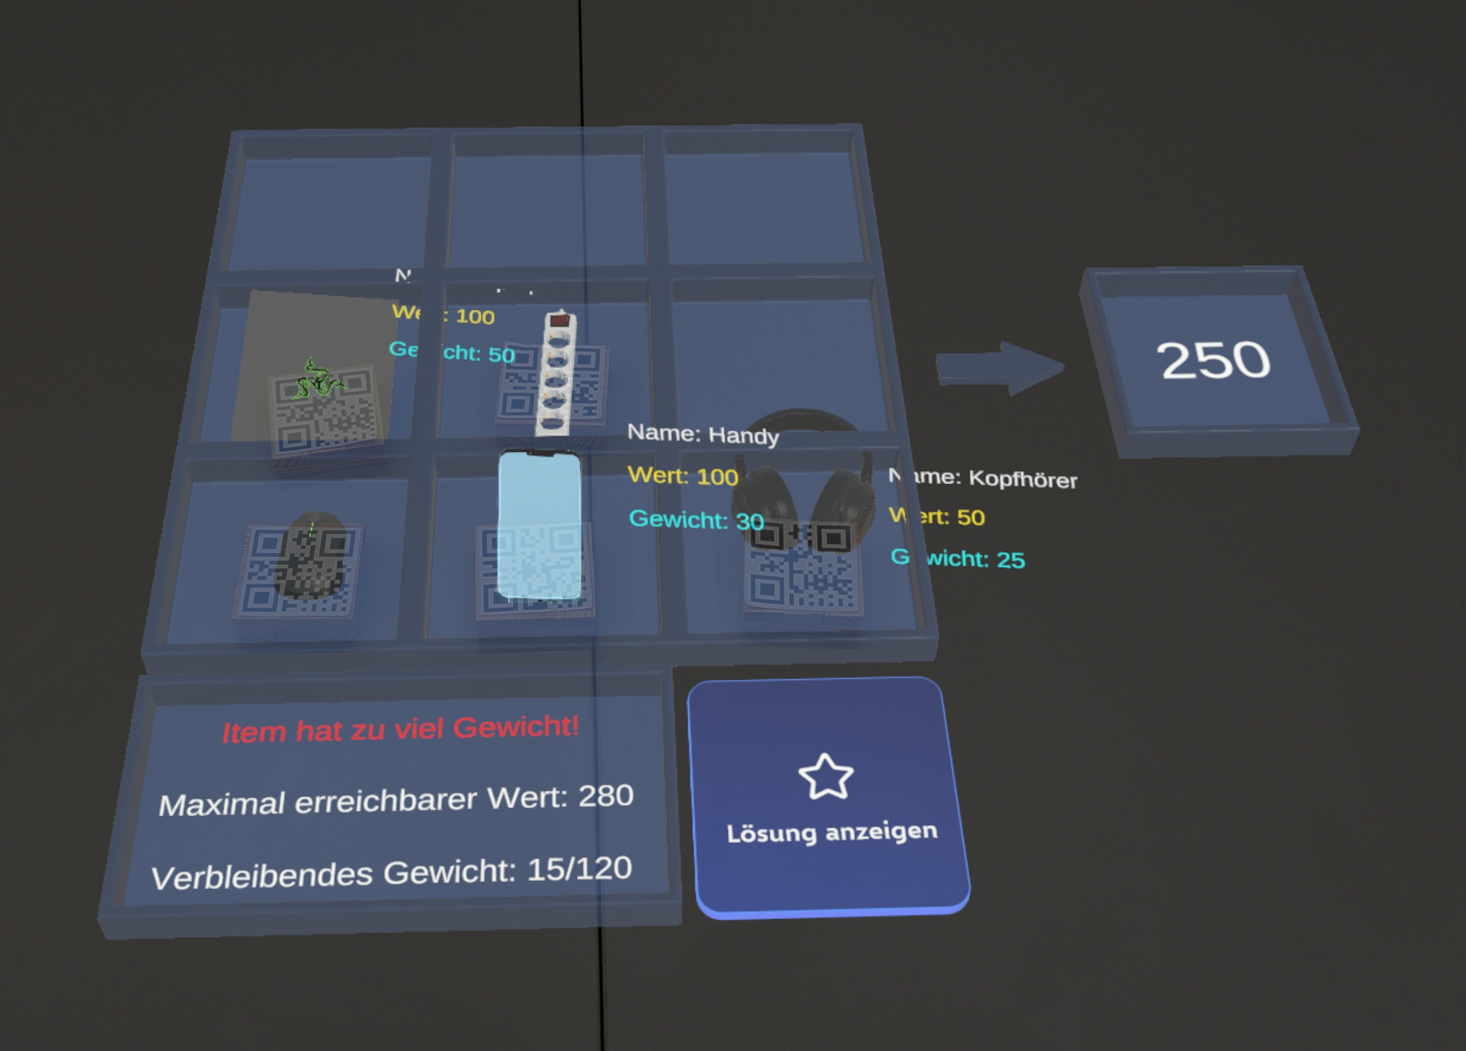
\includegraphics[scale=0.6]{images/itemToHeavy}
    \caption{Item zu schwer}
    \label{fig:controller_itemToHeavy}
\end{figure}

In Abbildung \ref{fig:controller_itemToHeavy} sind vier verschiedene Items im Inventar enthalten, mit den IDs
\textit{1, 3, 5, 9}. Die Reihenfolge ihres Hinzufügens zum Inventar war 1, 5, 9, 3. Das Item mit der ID 9 wurde jedoch
aufgrund seines zu hohen Gewichts nicht zu \textit{idGrid} und \textit{processedItems} hinzugefügt. Gleichzeitig wird
eine Fehlermeldung angezeigt, um dem Benutzer zu signalisieren, dass das zuletzt hinzugefügte Item zu schwer für das
aktuelle Inventar ist. Als Konsequenz bleiben \textit{idGrid} und \textit{processedItems} unverändert und enthalten
daher nicht die ID 9. Im Hintergrund sieht daher das \textit{idGrid} dementsprechend folgendermaßen aus:
\begin{lstlisting}[style=csharp, caption={Item zu schwer für das Inventar}, label=code:controller_savedIDs]
int idGrid = [[0, 0, 0],
              [5, 0, 0],
              [1, 3, 0]];
\end{lstlisting}\\
Das HashSet \textit{processedItems} sieht nach platzieren des Items dann so aus:
\begin{lstlisting}[style=csharp, caption={ID verspeichert}, label=code:controller_savedID]
processedItems = [1, 5, 9];
\end{lstlisting}\\
Sobald der Benutzer dieses Item wieder aus dem Inventar entfernt wird die Fehlermeldung nicht mehr angezeigt und es kann
ein passendes Item hinzugefügt werden.\\

Im alternativen Zweig der Hauptbedingung wird überprüft, ob das Item außerhalb der Inventargrenzen liegt, aber zuvor
als verarbeitet markiert wurde und weiterhin in \texttt{processedItems} und \texttt{idGrid} vorhanden ist. Dies deutet
darauf hin, dass das Item aus dem Inventar entfernt wurde. In diesem Fall wird die ID des Items aus \texttt{processedItems}
und \texttt{idGrid} entfernt, und das Gewicht des Inventars wird entsprechend angepasst. Auch hier wird ein
\texttt{GridUpdate}-Ereignis ausgelöst.\\

\begin{figure}[h]
    \centering
    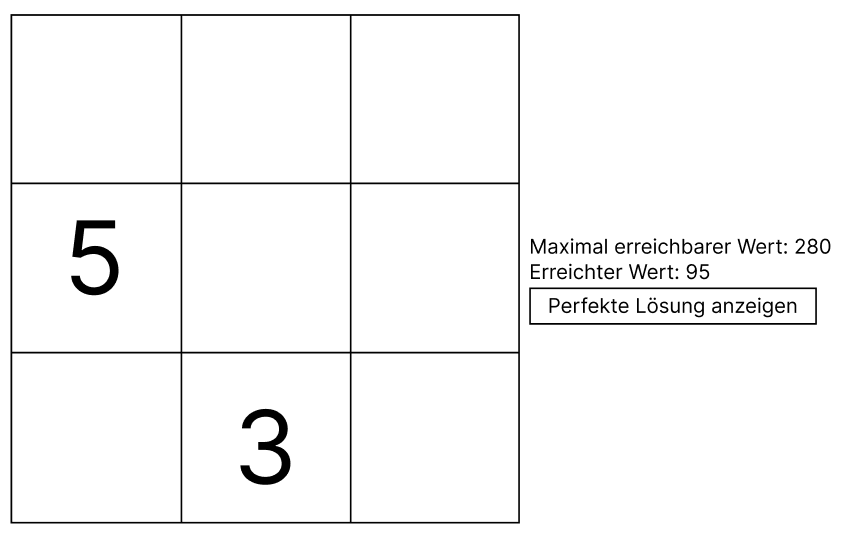
\includegraphics[scale=0.6]{images/itemEntfernt}
    \caption{Item aus Inventar entfernt}
    \label{fig:controller_itemEntfernt}
\end{figure}

In Abbilding \ref{fig:controller_itemEntfernt} ist der aktuelle Zustand eines selbst zusamengestellten Inventars zu sehen. In
diesem Inventar sind die beiden Items mit den IDs \textit{5, 3} enthalten. Im Hintergrund sieht das \textit{idGrid} jedoch so aus:
\begin{lstlisting}[style=csharp, caption={ID trotz nicht vorhandenem Item gespeichert}, label=code:controller_savedIDitemEntferntGrid]
int idGrid = [[0, 0, 0],
              [5, 0, 0],
              [1, 3, 0]];
\end{lstlisting}\\
Und das HashSet \textit{processedItems} sieht so aus:
\begin{lstlisting}[style=csharp, caption={ID trotz nicht vorhandenem Item gespeichert}, label=code:controller_savedIDItemEntferntHash]
processedItems = [1, 5, 3];
\end{lstlisting}\\
Anhand der Abbildung \ref{fig:controller_itemEntfernt} und den beiden Codeabschnitten \ref{code:controller_savedIDitemEntferntGrid}
und \ref{code:controller_savedIDItemEntferntHash} ist aber zu sehen, dass hier noch die ID \textit{1} gespeichert ist.
Dies bedeutet, dass das Item mit der ID \textit{1} in einem vorherigen Zustand im Inventar platziert wurde aber jetzt außerhalb
der Bounds des Iventars liegt. Anhand dieser Erkenntnis wird anschließend diese ID aus dem \textit{idGrid} und \textit{processedItems}
entfernt und das \textit{currWeight} angepasst. Diese sehen nach der Entfernung dieser ID folgendermaßen aus:
\begin{lstlisting}[style=csharp, caption={ID trotz nicht vorhandenem Item gespeichert}, label=code:controller_savedIDgg]
int idGrid = [[0, 0, 0],
              [5, 0, 0],
              [0, 3, 0]];
\end{lstlisting}
\begin{lstlisting}[style=csharp, caption={ID verspeichert}, label=code:controller_savedIDID]
processedItems = [5, 3];
\end{lstlisting}\\
Schließlich erfolgt der Aufruf der Funktion \textbf{PrintGrid()}, die Testweise für das Debugging enthalten ist
um aus den Logs herauslesen zu können, wie das \textit{idGrid} aufgebaut ist und welche Items enthalten sind und ob
die Berechnung und Platzierung richtig abgelaufen ist.

\subsubsection{Berechnen der Position im idGrid anhand der Koordinaten}
In Codeabschnitt \ref{code:controller_check} wird bei platzieren eines Items innerhalb des Inventars die Funktion
\textbf{CalculateGridPosition()} aufgerufen. Diese Funktion kümmert sich darum, dass anhand der gegebenen Koordinaten des
Items innerhalb des Inventar Modells ein Vektor Berechnet wird an welcher Stelle dieses Item im \textit{idGrid} liegt.
Diese Funktion sieht folgendermaßen aus:
\begin{lstlisting}[style=csharp, caption={Stelle im idGrid anhand Koordinaten berechnen}, label=code:controller_calcPos]
private Vector2 CalculateGridPosition(Vector3 objectPosition)
{
    float cellWidth = inventoryBounds.size.x / numColumns;
    float cellHeight = inventoryBounds.size.z / numRows;
    int col = Mathf.FloorToInt((objectPosition.x - inventoryBounds.min.x) / cellWidth);
    int row = Mathf.FloorToInt((inventoryBounds.max.z - objectPosition.z) / cellHeight);
    return new Vector2(row, col);
}
\end{lstlisting}\\
Die Funktion beginnt damit, dass sie sich anhand der Länge der Bounds in X- und Y-Achse die Länge einer einzelnen Zelle
berechnet. Die Variable \texttt{cellWidth} repräsentiert die Breite jeder Zelle, und \texttt{cellHeight} repräsentiert
die Höhe jeder Zelle im Inventar-Raster.

Anschließend werden die 2D-Koordinaten der Position des übergebenen Objekts im Inventar-Raster berechnet. Dazu wird
zuerst die X-Koordinate des Objekts relativ zur minimalen X-Grenze der Inventar-Bounds genommen und durch die Breite
einer Zelle (\texttt{cellWidth}) geteilt. Dieser Wert wird dann auf die nächste ganze Zahl abgerundet
(\texttt{Mathf.FloorToInt}) und repräsentiert die Spalte (\texttt{col}) im Raster.

Ebenso wird die Z-Koordinate des Objekts relativ zur maximalen Z-Grenze der Inventar-Bounds genommen und durch die Höhe
einer Zelle (\texttt{cellHeight}) geteilt. Auch dieser Wert wird auf die nächste ganze Zahl abgerundet und repräsentiert
die Zeile (\texttt{row}) im Raster.

Abschließend werden die berechneten Zeilen- und Spaltenwerte als 2D-Vektor (\texttt{Vector2}) zurückgegeben, der die
Position des Objekts im Inventar-Raster repräsentiert.

\subsubsection{Hilfsfunktionen}
Im Codeabschnitt \ref{code:controller_check} werden die Funktionen \textbf{RemoveItem} und \textbf{ContainsID} für die
Entfernung eines Items aus dem \textit{idGrid} und die Überprüfung, ob eine bestimmte Item-ID im \textit{idGrid}
vorhanden ist, verwendet. Die Funktion \textbf{RemoveItem} hat den Zweck, ein Item anhand seiner ID aus dem \textit{idGrid} zu entfernen.
Die Funktion \textbf{ContainsID} wird verwendet, um zu überprüfen, ob eine bestimmte Item-ID bereits im \textit{idGrid}
vorhanden ist. Die Implementierungen dieser Funktionen sind entsprechend:
\begin{lstlisting}[style=csharp, caption={ID aus idGrid entfernen}, label=code:controller_removeID]
private void RemoveItem(int id)
{
    for (int i = 0; i < numRows; i++)
    {
        for (int j = 0; j < numColumns; j++)
        {
            if (idGrid[i, j] == id)
            {
                idGrid[i, j] = 0;
                return;
            }
        }
    }
}
\end{lstlisting}\\
\begin{lstlisting}[style=csharp, caption={Ueberpruefen ob ID in idGrid enthalten ist}, label=code:controller_contains ID]
private bool ContainsId(int id)
{
    for (int i = 0; i < numRows; i++)
    {
        for (int j = 0; j < numColumns; j++)
        {
            if (idGrid[i, j] == id)
            {
                return true;
            }
        }
    }
    return false;
}
\end{lstlisting}\\

\subsection{Knapsack Algorithmus Definition}
Im folgenden Abschnitt wird der Knapsack-Algorithmus allgemein erklärt, die Problemstellung verdeutlicht und die
Unterschiede der beiden möglichen Algorithmen erläutert. Außerdem wird darauf eingegangen, warum er so wichtig ist
und in welchen Anwendungen er zum Einsatz kommt.

Der Knapsack-Algorithmus ist ein häufig verwendetes Werkzeug in der Informatik, um das Problem der optimalen
Ressourcenallokation zu lösen. Dieses Problem tritt auf, wenn eine begrenzte Menge an Ressourcen so effizient wie
möglich genutzt werden soll, um einen bestimmten Nutzen oder Gewinn zu maximieren. Der Begriff "Knapsack" leitet sich
von der Idee ab, dass man versucht, einen Rucksack mit begrenztem Fassungsvermögen mit Gegenständen zu füllen, die
unterschiedliche Werte und Gewichte haben.

\subsubsection{Problemstellung}
Gegeben sei ein Rucksack mit begrenzter Kapazität und eine Menge von Gegenständen, von denen jeder einen bestimmten
Wert und ein bestimmtes Gewicht hat. Das Ziel besteht darin, die Gegenstände auszuwählen, die in den Rucksack passen
und den Gesamtwert maximieren.

\subsubsection{Algorithmus}
Der Knapsack-Algorithmus kann in verschiedenen Varianten implementiert werden, darunter der dynamische
Programmieransatz und der Greedy-Ansatz. Im dynamischen Programmieransatz wird eine Tabelle erstellt, um
Teilprobleme zu lösen und die optimale Lösung zu berechnen. Der Greedy-Ansatz hingegen wählt Gegenstände basierend
auf bestimmten Kriterien aus, um eine lokale Optimierung zu erreichen.

In unserem Kontext wurde der dynamische Programmieransatz implementiert, um den Knapsack-Algorithmus umzusetzen.
Der Code dafür ist in der Datei \textit{KnapsackScript.cs} zu finden, welche den maximal erreichbaren Wert und
die optimale Lösung berechnet.

\subsubsection{Anwendungen}
Der Knapsack-Algorithmus findet Anwendung in verschiedenen Bereichen, darunter Logistik, Finanzplanung,
Ressourcenmanagement und Netzwerkoptimierung. Beispielsweise kann er verwendet werden, um den effizientesten
Transport von Gütern mit begrenzten Kapazitäten zu planen oder in der Finanzplanung, um das Portfolio von
Investitionen zu optimieren.

\subsection{Knapsack Algorithmus Implementierung}
Der folgende Abschnitt beschreibt das \textit{KnapsackScript.cs} und den darin geschriebenen Code für die Umsetzung des
dynamischen Knapsack-Algorithmus in C-Sharp unter Verwendung von Unity. Die Implementierung umfasst den Funktionsaufruf, die
Initialisierung der Variablen für den Algorithmus, den eigentlichen Algorithmus, das Backtracking zur
Identifizierung der ausgewählten Gegenstände für die perfekte Lösung, die Berechnung der Gruppengröße, die Konvertierung
der temporären Liste in ein 2D-Array, die Rückgabe des Gesamtwerts, sowie die Darstellung der perfekten Lösung und die
Berechnung des eigenen Inventars.

\subsubsection{Funktionsaufruf}
\begin{lstlisting}[style=csharp, caption={}, label=code:init]
int maxValue = KnapsackMaxValue(out usedItems, out int coveredCapacity);
int inventoryValue = -1;
maxMesh.text = "Maximal erreichbarer Wert: " + maxValue.ToString();
\end{lstlisting}
\textbf{Erklärung:} In diesem Codeabschnitt erfolgt der Aufruf der Funktion \textit{KnapsackMaxValue}. Die beiden
\textit{out}-Parameter (\textit{usedItems} und \textit{coveredCapacity}) dienen dazu, Werte aus der Funktion
herauszugeben, und werden nach dem Funktionsaufruf mit den berechneten Werten aktualisiert. Der Rückgabewert
\textit{maxValue} enthält den maximal erreichbaren Wert des Rucksacks. Dieser Wert wird dann im TextMesh \textit{maxMesh}
dargestellt, um dem Benutzer die Information über den maximal erreichbaren Wert anzuzeigen.

\subsubsection{Initialisierung der Variablen für den Algorithmus}
\begin{lstlisting}[style=csharp, caption={}, label=code:variable]
int n = items.Count;
int[,] dp = new int[n + 1, capacity + 1];
bool[,] selected = new bool[n + 1, capacity + 1];
\end{lstlisting}
\textbf{Erklärung:} Die Initialisierung erstellt die notwendigen Arrays für die dynamische Programmierung.\\

\subsubsection{Dynamischer Knapsack Algorithmus}
\begin{lstlisting}[style=csharp, caption={}, label=code:dynamic]
for (int i = 0; i <= n; i++)
{
    for (int w = 0; w <= capacity; w++)
    {
        % Initialisierung der DP-Tabelle
        if (i == 0 || w == 0)
            dp[i, w] = 0;
        else if (items[i].weight <= w && i <= maxItems)
        {
            % Berechnung des neuen Werts, wenn das Item ausgewählt wird
            int newValue = items[i].value + dp[i - 1, w - items[i].weight];
            if (newValue > dp[i - 1, w])
            {
                dp[i, w] = newValue;
                selected[i, w] = true;
            }
            else
            {
                dp[i, w] = dp[i - 1, w];
                selected[i, w] = false;
            }
        }
        else
        {
            dp[i, w] = dp[i - 1, w];
            selected[i, w] = false;
        }
    }
}
\end{lstlisting}

\textbf{Erklärung:}
\begin{enumerate}
    \item \textbf{Iterationen durch die Items und Kapazität:} Die äußere Schleife durchläuft jedes Item
    (\texttt{i}) von 0 bis zur Gesamtanzahl der Items (\texttt{n}). Die innere Schleife durchläuft jede mögliche
    Kapazität (\texttt{w}) von 0 bis zur maximalen Kapazität des Rucksacks.

    \item \textbf{Initialisierung der DP-Tabelle:} Wenn \texttt{i} oder \texttt{w} 0 ist, wird der Wert in der
    DP-Tabelle auf 0 gesetzt. Dies liegt daran, dass es keine Items gibt oder die Kapazität des Rucksacks 0 ist.

    \item \textbf{Überprüfung, ob das Item ausgewählt werden kann:} Wenn das aktuelle Item ausgewählt werden
    kann (basierend auf Gewicht und maximaler Anzahl von Items), wird der neue Wert berechnet, wenn das Item
    ausgewählt wird.

    \item \textbf{Vergleich und Auswahl:} Der neue Wert wird mit dem Wert verglichen, wenn das Item nicht
    ausgewählt wird. Wenn der neue Wert größer ist, wird das Item ausgewählt (\texttt{selected[i, w] = true}),
    andernfalls wird das vorherige Ergebnis beibehalten (\texttt{selected[i, w] = false}).

    \item \textbf{Falls Item nicht ausgewählt wird:} Wenn das aktuelle Item nicht ausgewählt wird, wird der
    Wert in der DP-Tabelle auf den Wert gesetzt, den das Rucksack ohne das aktuelle Item in der vorherigen
    Iteration erreicht hat.\\
\end{enumerate}

\textbf{Bedeutung der DP-Tabelle:}
Die DP-Tabelle (dp) dient dazu, Teilprobleme zu lösen und die besten Ergebnisse für verschiedene Kombinationen
von Items und Kapazitäten zu speichern. Jeder Eintrag in der Tabelle repräsentiert den maximal erreichbaren Wert
für eine bestimmte Menge von ausgewählten Items und eine bestimmte Kapazität des Rucksacks.

Insgesamt ermöglicht dieser Algorithmus, die optimale Auswahl von Gegenständen zu finden, die in den Rucksack
passt, um den Gesamtwert zu maximieren.


\subsubsection{Backtracking, um ausgewählte Items und perfekt Lösung zu finden}
\begin{lstlisting}[style=csharp, caption={}, label=code:backtrack]
List<List<int>> tempUsedItems = new List<List<int>>();
int row = n;
int col = capacity;
while (row > 0 && col > 0)
{
    List<int> group = new List<int>();
    while (row > 0 && col > 0 && selected[row, col])
    {
        // Item zu ausgewählter Gruppe hinzufügen
        group.Add(items[row].id);
        col -= items[row].weight;
        row--;
    }

    // Hinzufügen der Gruppe zur Liste
    if (group.Count > 0)
    {
        tempUsedItems.Add(group);
    }

    // Fortfahren mit dem Backtracking
    if (row > 0 && col > 0)
    {
        row--;
    }
}
\end{lstlisting}

\textbf{Erklärung:}
\begin{enumerate}
    \item \textbf{Initialisierung von Zeilen- und Spaltenindizes:} Die Variablen \texttt{row} und \texttt{col} werden auf die letzte Zeile und Spalte der DP-Tabelle gesetzt.

    \item \textbf{Hauptschleife für Backtracking:} Die äußere Schleife wird durchlaufen, solange die Zeile und die Spalte größer als 0 sind.

    \item \textbf{Innere Schleife für Gruppenbildung:} Solange die Zeile und die Spalte größer als 0 sind und das Item in der DP-Tabelle ausgewählt wurde (\texttt{selected[row, col]}), wird das Item zur aktuellen Gruppe hinzugefügt, das Gewicht von der aktuellen Kapazität abgezogen, und die Zeile wird dekrementiert.

    \item \textbf{Hinzufügen der Gruppe zur Liste:} Wenn die Gruppe mindestens ein Item enthält, wird die Gruppe zur temporären Liste \texttt{tempUsedItems} hinzugefügt.

    \item \textbf{Fortfahren mit dem Backtracking:} Die Zeile wird dekrementiert, um das nächste ausgewählte Item zu finden.
\end{enumerate}

Diese Schritte werden wiederholt, bis alle ausgewählten Items gefunden sind und die temporäre Liste \texttt{tempUsedItems} alle ausgewählten Gruppen enthält.\\

\subsubsection{Gruppengröße berechnen}
\begin{lstlisting}[style=csharp, caption={}, label=code:maxgroup]
int maxGroupSize = 0;
foreach (var group in tempUsedItems)
{
    if (group.Count > maxGroupSize)
        maxGroupSize = group.Count;
}
\end{lstlisting}
\textbf{Erklärung:} Findet die maximale Gruppengröße.\\

\subsubsection{Temporäres Array umwandeln und das usedItems Array befüllen}
\begin{lstlisting}[style=csharp, caption={}, label=code:convert]
usedItems = new int[tempUsedItems.Count, maxGroupSize];
for (int i = 0; i < tempUsedItems.Count; i++)
{
    for (int j = 0; j < tempUsedItems[i].Count; j++)
    {
        usedItems[i, j] = tempUsedItems[i][j];
    }
}
\end{lstlisting}
\textbf{Erklärung:} Konvertiert die temporäre Liste von Gruppen in ein 2D-Array, um die ausgewählten Items also die perfekt Lösung zu speichern.\\

\subsubsection{Rückgabewert}
\begin{lstlisting}[style=csharp, caption={}, label=code:return]
return dp[n, capacity];
\end{lstlisting}
\textbf{Erklärung:} Gibt den Gesamtwert des besten Rucksacks zurück.\\

\subsubsection{Darstellung der perfekten Lösung}
Um die perfekt Lösung nach der Berechnung erfolgreich darzustellen wird in diesem Abschnitt auf die \texit{PLACEHOLDES} Funktion des
\textit{KnapsackScript.cs} eingegangen um die errechnete Lösung nach dem drücken des \textit{SolveButton} anzugeigen

\subsubsection{Berechnen des eigenen Inventars}
In diesem Abschnitt wird auf die Funktion \textit{KnapsackInventoryValue} des \texit{KnapsackScript.cs} eingegangen. Diese Funktion
berechnet das Inventar Value des selbst gebauten Inventars.

\subsubsection{Funktionsaufruf}
\begin{lstlisting}[style=csharp, caption={}, label=code:aufruf]
inventoryValue = KnapsackInventoryValue(inventory);
if (maxValue == inventoryValue)
{
    infoMesh.color = Color.green;
    infoMesh.text = "Maximale Punktzahl erreicht";
}
else
{
    infoMesh.text = "";
}
ownMesh.text = "Erreichter Wert: " + inventoryValue.ToString();
\end{lstlisting}
\textbf{Erklärung:}
\begin{enumerate}
    \item \textbf{Inventar Wert berechnen:} Die Funktion KnapsackInventoryValue wird mit dem übergebenem invetory aufgerufen und der Inventar Wert berechnet.
    \item \textbf{Ergebnis Handling:} Wenn der eigene Wert gleich dem Maximalen errechnetem Wert enspricht hat der Benutzer gewonnen. Anderenfalls wird dem \texit{infoMesh} der aktuelle Wert zugewiesen.
\end{enumerate}

\subsubsection{Code für die Berechnung des eigenen Inventars}
\begin{lstlisting}[style=csharp, caption={}, label=code:ownInventory]
int KnapsackInventoryValue(int[,] inventory)
{
    if(inventory == null)
    {
        throw new System.Exception("Inventory is null");
    }

    int totalValue = 0;

    foreach (var item in items.Values)
    {
        int itemId = item.id;
        int itemValue = item.value;

        for (int j = 0; j < inventory.GetLength(0); j++)
        {
            for (int k = 0; k < inventory.GetLength(1); k++)
            {
                if (inventory[j, k] == itemId)
                {
                    totalValue += itemValue;
                }
            }
        }
    }

    return totalValue;
}
\end{lstlisting}
\textbf{Erklärung:}
\begin{enumerate}
    \item \textbf{Überprüfung auf Null:} Die Funktion überprüft, ob das übergebene Inventar null ist. Falls ja, wird eine Ausnahme ausgelöst.

    \item \textbf{Initialisierung des Gesamtwerts:} Die Variable \texttt{totalValue} wird auf 0 initialisiert. Hier wird der Gesamtwert des Rucksackinventars gespeichert.

    \item \textbf{Durchlauf aller Gegenstände:} Die Funktion durchläuft alle Gegenstände im globalen \texttt{items}-Dictionary.

    \item \textbf{Extrahierung von Informationen:} Für jeden Gegenstand werden die ID (\texttt{itemId}) und der Wert (\texttt{itemValue}) extrahiert.

    \item \textbf{Durchlauf des Inventars:} Die doppelte Schleife durchläuft das gesamte Inventar (\texttt{inventory}) und prüft, ob der aktuelle Gegenstand vorhanden ist.

    \item \textbf{Berechnung des Gesamtwerts:} Wenn der Gegenstand im Inventar gefunden wird, wird sein Wert zum Gesamtwert (\texttt{totalValue}) addiert.

    \item \textbf{Rückgabe des Gesamtwerts:} Am Ende wird der Gesamtwert des Rucksackinventars zurückgegeben.
\end{enumerate}

\subsection{Unit-Tests}
Durch Hilfe von Unit-Tests wird versichert, dass der implementierte Knappsack-Algorithmus
richtig und performant funktioniert.
%Genauere Erklärung + Custom Code der UnitTests

\section{Performance}
Performance-Messung
